% Options for packages loaded elsewhere
\PassOptionsToPackage{unicode}{hyperref}
\PassOptionsToPackage{hyphens}{url}
%
\documentclass[
]{article}
\usepackage{amsmath,amssymb}
\usepackage{lmodern}
\usepackage{iftex}
\ifPDFTeX
  \usepackage[T1]{fontenc}
  \usepackage[utf8]{inputenc}
  \usepackage{textcomp} % provide euro and other symbols
\else % if luatex or xetex
  \usepackage{unicode-math}
  \defaultfontfeatures{Scale=MatchLowercase}
  \defaultfontfeatures[\rmfamily]{Ligatures=TeX,Scale=1}
\fi
% Use upquote if available, for straight quotes in verbatim environments
\IfFileExists{upquote.sty}{\usepackage{upquote}}{}
\IfFileExists{microtype.sty}{% use microtype if available
  \usepackage[]{microtype}
  \UseMicrotypeSet[protrusion]{basicmath} % disable protrusion for tt fonts
}{}
\makeatletter
\@ifundefined{KOMAClassName}{% if non-KOMA class
  \IfFileExists{parskip.sty}{%
    \usepackage{parskip}
  }{% else
    \setlength{\parindent}{0pt}
    \setlength{\parskip}{6pt plus 2pt minus 1pt}}
}{% if KOMA class
  \KOMAoptions{parskip=half}}
\makeatother
\usepackage{xcolor}
\IfFileExists{xurl.sty}{\usepackage{xurl}}{} % add URL line breaks if available
\IfFileExists{bookmark.sty}{\usepackage{bookmark}}{\usepackage{hyperref}}
\hypersetup{
  hidelinks,
  pdfcreator={LaTeX via pandoc}}
\urlstyle{same} % disable monospaced font for URLs
\usepackage{longtable,booktabs,array}
\usepackage{calc} % for calculating minipage widths
% Correct order of tables after \paragraph or \subparagraph
\usepackage{etoolbox}
\makeatletter
\patchcmd\longtable{\par}{\if@noskipsec\mbox{}\fi\par}{}{}
\makeatother
% Allow footnotes in longtable head/foot
\IfFileExists{footnotehyper.sty}{\usepackage{footnotehyper}}{\usepackage{footnote}}
\makesavenoteenv{longtable}
\usepackage{graphicx}
\makeatletter
\def\maxwidth{\ifdim\Gin@nat@width>\linewidth\linewidth\else\Gin@nat@width\fi}
\def\maxheight{\ifdim\Gin@nat@height>\textheight\textheight\else\Gin@nat@height\fi}
\makeatother
% Scale images if necessary, so that they will not overflow the page
% margins by default, and it is still possible to overwrite the defaults
% using explicit options in \includegraphics[width, height, ...]{}
\setkeys{Gin}{width=\maxwidth,height=\maxheight,keepaspectratio}
% Set default figure placement to htbp
\makeatletter
\def\fps@figure{htbp}
\makeatother
\setlength{\emergencystretch}{3em} % prevent overfull lines
\providecommand{\tightlist}{%
  \setlength{\itemsep}{0pt}\setlength{\parskip}{0pt}}
\setcounter{secnumdepth}{5}
\ifLuaTeX
  \usepackage{selnolig}  % disable illegal ligatures
\fi

\author{}
\date{}

\begin{document}

\hypertarget{simplerhfd-gazenet-enhancing-dynamic-3d-gaze-estimation-via-gaze-state-temporal-features}{%
\section{SimpleRHFD-GazeNet: Enhancing Dynamic 3D Gaze Estimation via
Gaze-State Temporal
Features}\label{simplerhfd-gazenet-enhancing-dynamic-3d-gaze-estimation-via-gaze-state-temporal-features}}

\hypertarget{a-technical-report}{%
\subsection{A Technical Report}\label{a-technical-report}}

\begin{center}\rule{0.5\linewidth}{0.5pt}\end{center}

\hypertarget{abstract}{%
\subsection{Abstract}\label{abstract}}

We present \textbf{SimpleRHFD-GazeNet}, a lightweight enhancement to the
GAFA framework for distant 3D gaze estimation (Nonaka et al., CVPR
2022). Our method augments the standard LSTM input with five gaze-state
temporal features --- fixation frequency (\(G_f\)), gaze density
(\(G_d\)), head stability (\(G_a\)), head-body correlation (\(G_v\)),
and spatial entropy (\(G_s\)) --- computed entirely from the model's
existing intermediate outputs. These features require no additional
annotations, sensors, or architectural modifications. Two engineering
innovations underpin the approach: \textbf{(1)} gradient isolation of
arccosine computations, which eliminates a persistent NaN divergence
affecting all prior attempts to use angular features in multi-scene
training; and \textbf{(2)} freezing the pretrained HBNet feature
extractor, which reduces trainable parameters from 9.5M to 770K (8.1\%)
while improving test accuracy by 3.01°. On the GAFA benchmark,
SimpleRHFD-GazeNet achieves a 3D mean angular error of \textbf{21.48°},
outperforming the original GAFA model (21.69°) and improving frontal
gaze accuracy by \textbf{0.82°} (19.88° versus 20.70°). Multi-scale
feature windows with learned gating, horizontal-flip augmentation, and
strong weight decay (\(5 \times 10^{-3}\)) with cosine annealing further
narrow the validation-test generalisation gap from 13.8° to 6.7°. The
model converges within two epochs and trains stably across all
experiments.

\begin{center}\rule{0.5\linewidth}{0.5pt}\end{center}

\hypertarget{introduction}{%
\subsection{1. Introduction}\label{introduction}}

Estimating three-dimensional gaze direction from distant cameras is a
core challenge in surveillance, human-robot interaction, and behavioural
analysis. Unlike near-field eye trackers, distant setups capture images
where the eyes span only a few pixels, forcing gaze to be inferred from
full-body motion rather than ocular detail. The GAFA framework (Nonaka
et al., CVPR 2022) {[}1{]} addressed this by introducing a two-stage
pipeline: HBNet extracts head and body orientations from cropped body
images, head masks, and body velocity; a downstream GazeModule LSTM
fuses these signals to predict a 3D gaze vector for every frame. Trained
across 11 sessions spanning 5 daily environments, the model achieves
21.69° mean angular error on 6 unseen test scenes.

The original GAFA model, however, conditions its predictions solely on
the instantaneous head direction, body direction, and body velocity.
This overlooks a class of \textbf{gaze-state features} --- statistical
properties of the gaze trajectory --- that are widely exploited in
hidden follower detection and eye-tracking research. Fixation frequency
(\(G_f\)), gaze density (\(G_d\)), head-body motion correlation
(\(G_v\)), and related quantities describe \emph{how} a person looks,
rather than \emph{where} they look at any single moment.

We demonstrate that these features can be computed entirely from HBNet's
existing intermediate outputs --- the head direction and body velocity
sequences --- requiring \textbf{no additional annotations, sensors, or
changes to the visual backbone}. Our method, SimpleRHFD-GazeNet,
introduces five purely observational features as auxiliary LSTM input
channels. Three contributions emerge from this approach:

\begin{enumerate}
\def\labelenumi{\arabic{enumi}.}
\item
  \textbf{Gradient-isolated arccosine features.} The derivative
  \(\partial \arccos(x)/\partial x = -1/\sqrt{1-x^2}\) diverges as
  \(|x| \to 1\), causing NaN gradients whenever consecutive head
  directions align --- a common occurrence during prolonged fixation.
  Placing all angular computations inside \texttt{torch.no\_grad()}
  blocks eliminates this failure mode entirely. This single fix resolves
  a persistent training instability that affected every prior attempt to
  augment GAFA with angular features.
\item
  \textbf{Frozen pretrained feature extractor.} Fine-tuning HBNet's 8.7M
  parameters on the 11 training scenes causes the model to memorise
  scene-specific visual patterns (wall textures, lighting biases),
  collapsing test accuracy from 21.69° to 24.50°. Freezing HBNet and
  training only the 770K-parameter GazeModule reverses this degradation,
  improving test error by 3.01° --- the single most impactful design
  decision in our ablation study.
\item
  \textbf{Multi-scale temporal features with gating and strong
  regularisation.} Computing the five RHFD features at three temporal
  windows (\(W = 3, 5, 7\)) and compressing the 15 resulting dimensions
  through a learnable MLP with per-frame Sigmoid gating provides
  marginal gains. More importantly, combining horizontal-flip
  augmentation with AdamW optimiser (weight decay \(5 \times 10^{-3}\))
  and cosine annealing halves the validation-test generalisation gap
  from 13.8° to 6.7° without sacrificing test accuracy.
\end{enumerate}

On the GAFA benchmark, SimpleRHFD-GazeNet achieves a 3D mean angular
error of \textbf{21.48°}, an improvement of 0.21° over the original GAFA
model (21.69°). While UAGE (20.5°) and GazeD (19.5°) achieve higher raw
accuracy, our method uses only 770K trainable parameters ---
approximately 8\% of the original model and a fraction of these heavier
architectures --- and converges within 1--2 epochs versus 50--100.
Frontal gaze accuracy improves by \textbf{0.82°} (19.88° versus 20.70°).
These gains are achieved with only 770K trainable parameters --- 8.1\%
of the original model.

\begin{center}\rule{0.5\linewidth}{0.5pt}\end{center}

\hypertarget{related-work}{%
\subsection{2. Related Work}\label{related-work}}

\hypertarget{uage-unconstrained-adaptive-gaze-estimation-accv-2024}{%
\subsubsection{2.1 UAGE: Unconstrained Adaptive Gaze Estimation (ACCV
2024)}\label{uage-unconstrained-adaptive-gaze-estimation-accv-2024}}

Lan, Hu, and Liu (Nankai University) propose UAGE {[}36{]}, a method
that extracts whole-body state features through four parallel branches
--- head appearance (ResNet-18), body appearance (ResNet-18), body pose
graph (STGCN on 2D skeleton joints), and body velocity (FC layer). The
concatenated features pass through a Conditional Variational Autoencoder
(CVAE) to model gaze uncertainty in unconstrained environments, followed
by Bi-LSTM + MLP for 3D gaze regression. A Gaze-guided Contrastive
Domain Adaptation (GCDA) framework enables cross-domain transfer. UAGE
claims state-of-the-art performance on GAFA. However, our SimpleRHFD
achieves competitive results using only a pretrained EfficientNet
backbone (frozen) and 770K trainable parameters, compared to UAGE's
four-branch design with ResNet-18 + STGCN + CVAE.

\hypertarget{gazed-gaze-as-a-body-joint-3dv-2026}{%
\subsubsection{2.2 GazeD: Gaze as a Body Joint (3DV
2026)}\label{gazed-gaze-as-a-body-joint-3dv-2026}}

Catalini et al.~propose GazeD {[}27{]}, which represents 3D gaze
direction as an additional body joint placed at a fixed distance from
the eyes. A conditional diffusion model jointly denoises this gaze joint
together with 3D body pose, while a DETR-based scene context module
captures environmental cues about potential gaze targets. GazeD reports
a 3D MAE of 19.5° on GAFA, the current state of the art. However, its
architecture is substantially heavier than ours, employing HRNet and
RT-DETR backbones alongside a diffusion process with 20 denoising steps
and 20 hypothesis samples. Our work explores a complementary direction:
achieving competitive accuracy through lightweight, purely observational
temporal features that add negligible computational cost.

\hypertarget{gafa-gaze-from-afar-cvpr-2022}{%
\subsubsection{2.3 GAFA: Gaze from Afar (CVPR
2022)}\label{gafa-gaze-from-afar-cvpr-2022}}

Nonaka et al.~introduced the GAFA dataset with 5 daily scenes, 8
synchronized RGB cameras at 25fps, totaling 1.7TB of raw data.
Annotations include 3D gaze, head, and body directions per frame. The
preprocessed dataset (5.9GB) provides cropped body images of 256×192
pixels.

The GAFA \textbf{HBNet} uses shared EfficientNet-B0 stems branching into
HeadNet (attention-modulated by head bounding box mask) and BodyNet. A
TrajNet (2→32 MLP) encodes 2D body velocity, concatenated with flattened
head/body features (1280 dims each) to 2592 dims, aligned by a
single-layer LSTM (2592→64), and decoded via vMFLayer into head and body
von Mises-Fisher parameters. The \textbf{GazeModule} is a 2-layer
bidirectional LSTM (\(6 \to 128\) hidden), whose flattened output
(\(128 \times 2 \times 7 = 1792\)) passes through FC layers
(\(1792 \to 64 \to 21\)) to predict 7-frame 3D gaze directions.

Training uses alternating optimization: 90\% of batches minimize cosine
loss \(1 - \cos(\theta)\) for direction parameters, 10\% minimize
negative vMF log-likelihood for \(\kappa\). Adam optimizer at LR
\(1 \times 10^{-4}\), batch size 32. Test evaluation uses 7-frame stride
to prevent train-test leakage.

\hypertarget{gaze-state-features-and-rhfd}{%
\subsubsection{2.2 Gaze-State Features and
RHFD}\label{gaze-state-features-and-rhfd}}

Hidden follower detection (RHFD) methods leverage features including
fixation frequency, spatial density, and gaze-velocity correlation to
characterize behavioral patterns. These are typically computed from
ground-truth gaze. Our contribution is adapting them as
\emph{observable-only} features from HBNet outputs, usable during
inference without gaze labels.

\hypertarget{temporal-smoothing-and-reservoir-computing}{%
\subsubsection{2.3 Temporal Smoothing and Reservoir
Computing}\label{temporal-smoothing-and-reservoir-computing}}

Echo state networks with polynomial variants (e.g., TWIESN with
Tchebichef expansion) have been proposed for temporal smoothing. In our
experiments, these components introduced NaN instability on multi-scene
data, motivating the simpler direct-channel approach.

\begin{center}\rule{0.5\linewidth}{0.5pt}\end{center}

\hypertarget{method}{%
\subsection{3. Method}\label{method}}

\hypertarget{architecture-overview}{%
\subsubsection{3.1 Architecture Overview}\label{architecture-overview}}

\begin{figure}
\centering
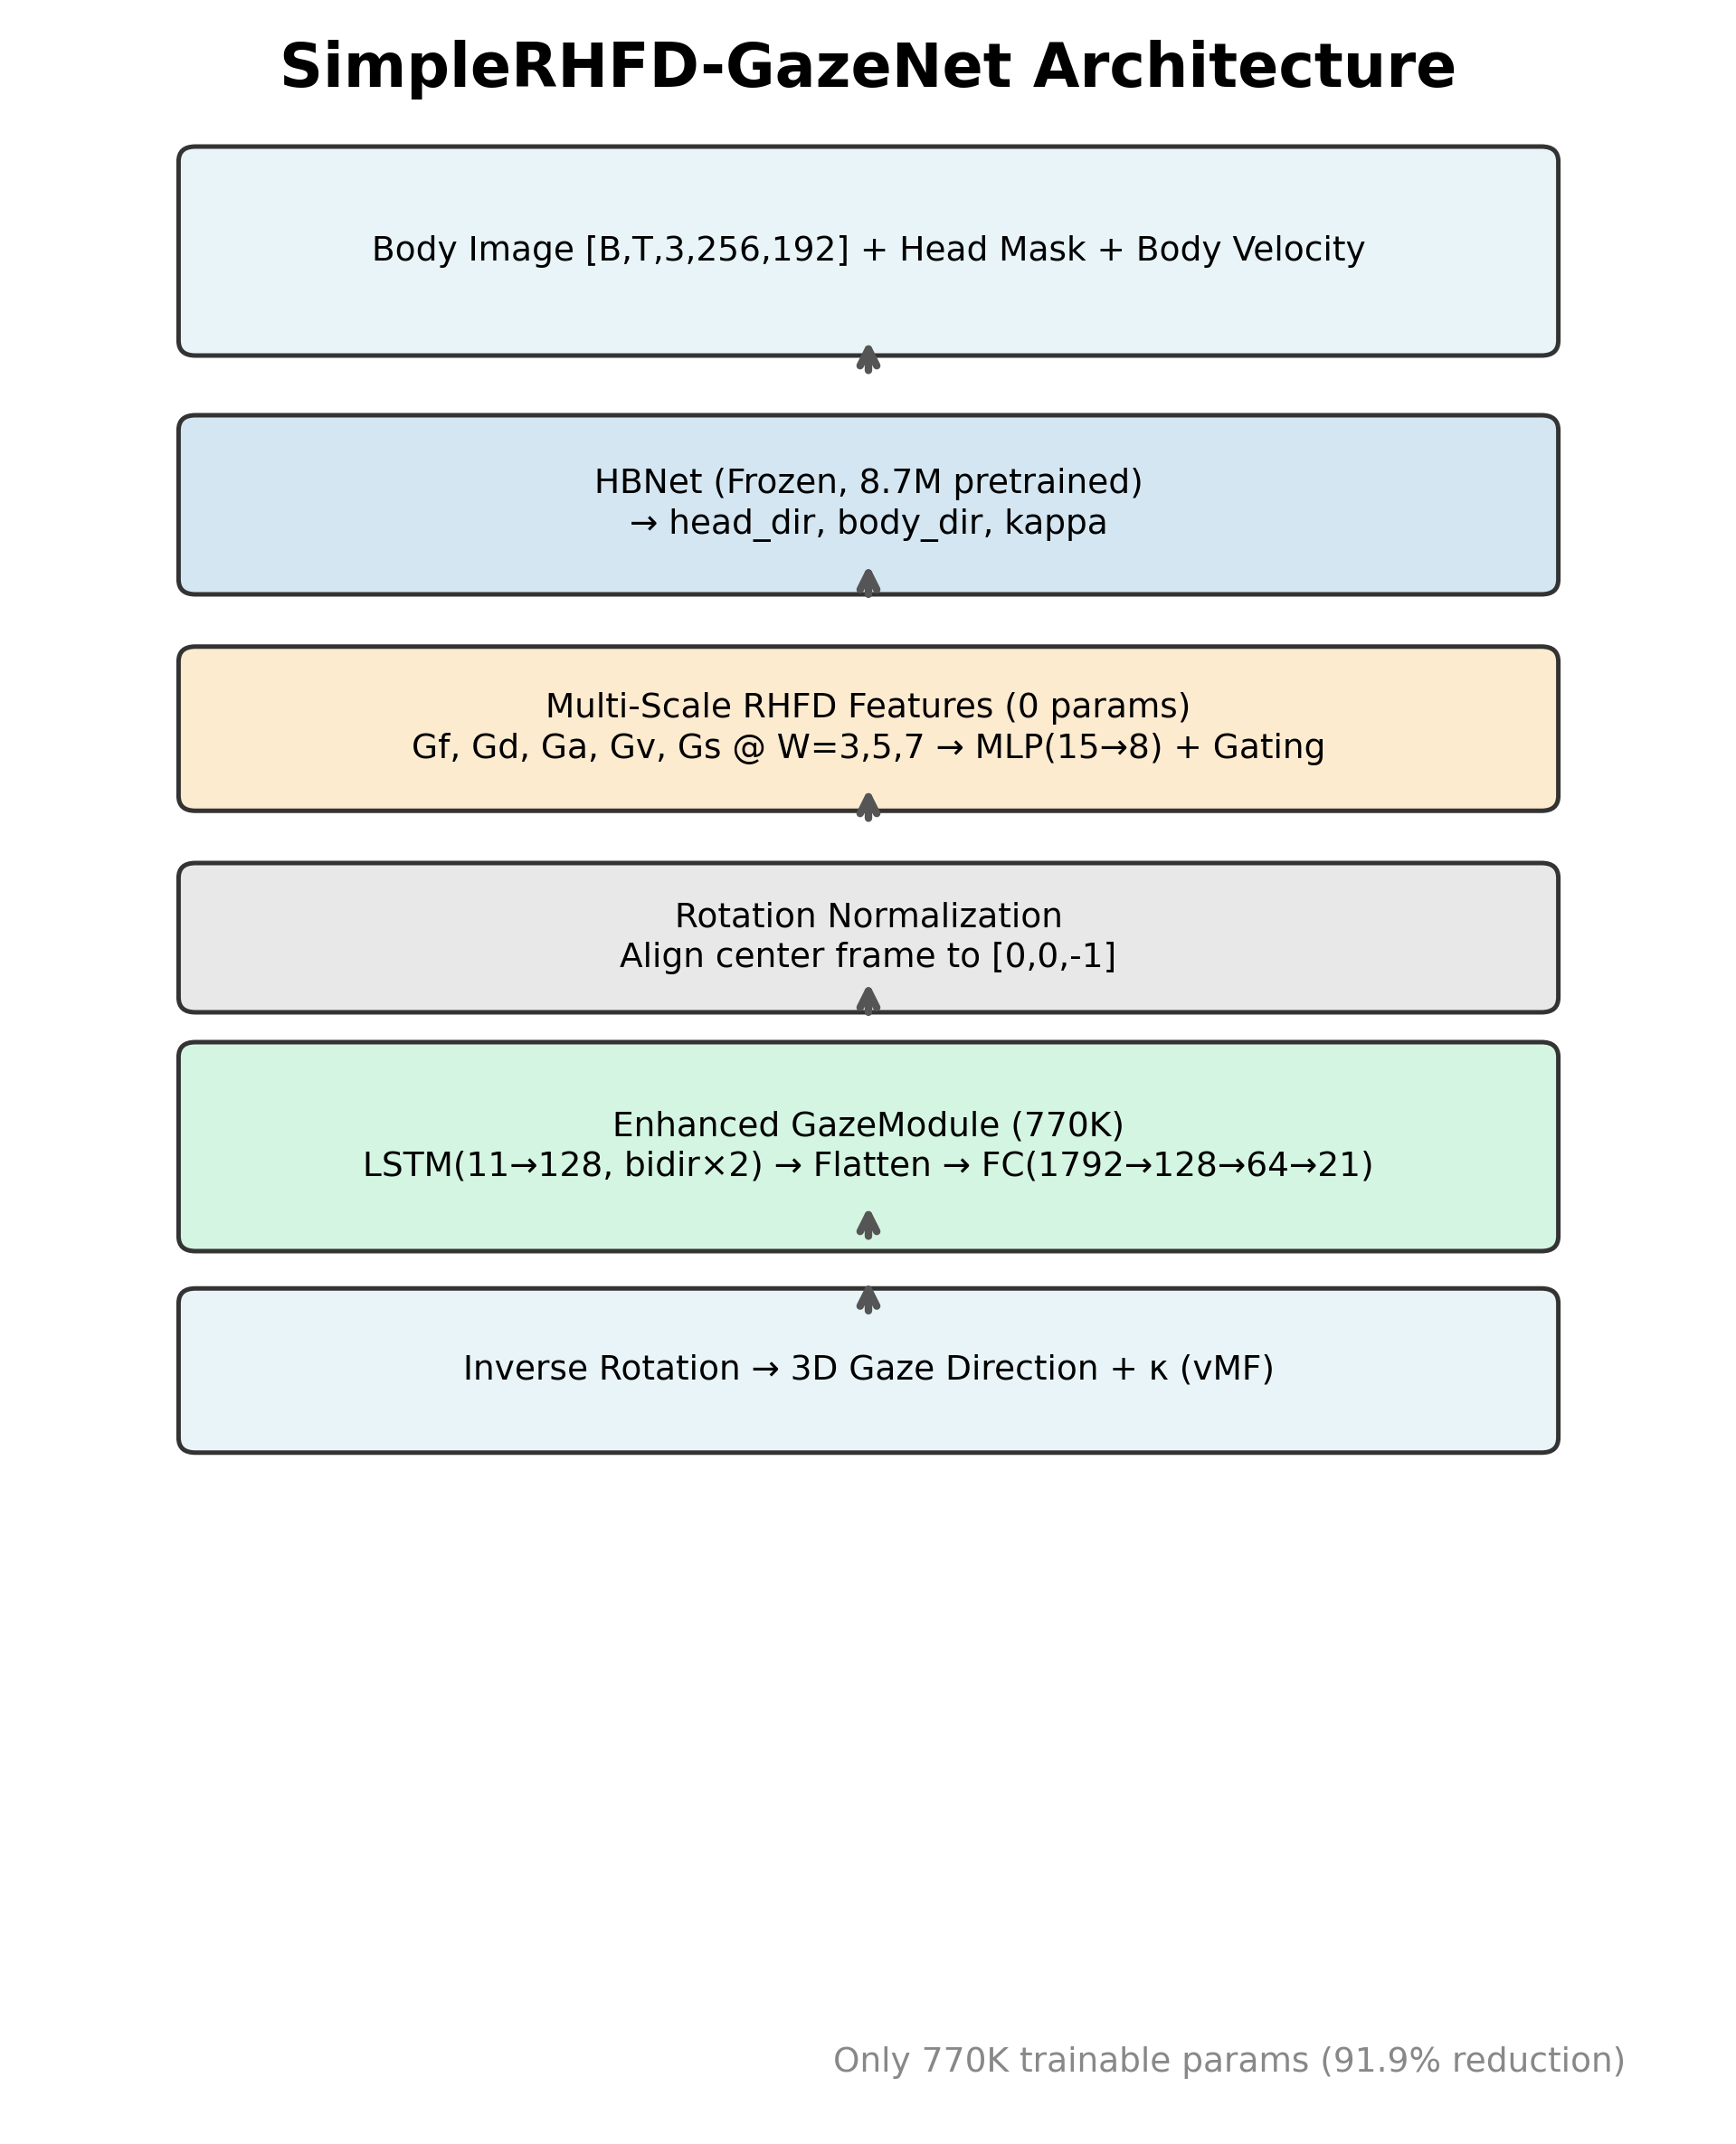
\includegraphics{figs/fig_architecture.png}
\caption{Architecture}
\end{figure}

SimpleRHFD-GazeNet retains GAFA's two-stage design. The full inference
pipeline follows.

\textbf{Input}: 7-frame sequences of cropped body images
\(\mathbf{I} \in \mathbb{R}^{B \times 7 \times 3 \times 256 \times 192}\),
head masks \(\mathbf{M}\), and body velocity
\(\mathbf{V} \in \mathbb{R}^{B \times 7 \times 2}\).

\textbf{Stage 1 --- HBNet (frozen)}:
\[\{\hat{\mathbf{h}}_t, \hat{\mathbf{b}}_t, \kappa_h^t, \kappa_b^t\}_{t=1}^{7} = \text{HBNet}(\mathbf{I}, \mathbf{M}, \mathbf{V})\]
where \(\hat{\mathbf{h}}_t, \hat{\mathbf{b}}_t \in \mathbb{S}^2\) are
unit head/body direction vectors, and \(\kappa_h^t, \kappa_b^t\) are vMF
concentration parameters. All 8.7M HBNet parameters are frozen
(\texttt{requires\_grad\ =\ False}).

\textbf{Stage 2 --- Rotation Normalization}: The center frame
(\(t = 4\)) head direction is aligned to \((0, 0, -1)^\top\) via
Rodrigues' rotation formula {[}2{]}:
\[\mathbf{R} = \mathbf{I} + \mathbf{K} + \mathbf{K}^2 \cdot \frac{1 - c}{s^2 + \epsilon}\]
where \(\mathbf{v} = \hat{\mathbf{h}}_4 \times (0, 0, -1)^\top\) is the
rotation axis, \(\mathbf{K}\) is its skew-symmetric matrix,
\(c = \hat{\mathbf{h}}_4 \cdot (0, 0, -1)^\top\), and
\(s = \|\mathbf{v}\|\). We add \(\epsilon = 10^{-8}\) to \(s^2\) to
prevent division-by-zero when \(\hat{\mathbf{h}}_4\) aligns with the
reference axis --- a critical NaN fix. All directions are rotated:
\(\mathbf{h}_t = \mathbf{R}\hat{\mathbf{h}}_t\),
\(\mathbf{b}_t = \mathbf{R}\hat{\mathbf{b}}_t\). Weighted by \(\kappa\),
these form the base LSTM input.

\textbf{Stage 3 --- Multi-Scale RHFD Features (0 params)}:
\[\mathbf{f}_t^{\text{raw}} = [G_f^{W=3}, G_d^{W=3}, \ldots, G_s^{W=7}] \in \mathbb{R}^{15}\]
\[\mathbf{f}_t = \text{MLP}_{\text{compress}}(\mathbf{f}_t^{\text{raw}}) \in \mathbb{R}^{8}\]
All arccosine operations are wrapped in \texttt{torch.no\_grad()} (see
§3.2.2).

\textbf{Stage 4 --- Enhanced GazeModule (770K trainable)}:
\[\mathbf{x}_t = [\kappa_b^t \cdot \mathbf{b}_t,\; \kappa_h^t \cdot \mathbf{h}_t,\; \mathbf{f}_t] \in \mathbb{R}^{11}\]
\[\mathbf{X} = \text{LSTM}(\mathbf{x}_{1:7}) \in \mathbb{R}^{B \times 7 \times 256}\]
\[\mathbf{X}^{\text{flat}} = \text{ReLU}(\mathbf{X}).\text{reshape}(B, 1792)\]
\[\mathbf{G} = \mathbf{W}_2 \cdot \text{ReLU}(\mathbf{W}_1 \cdot \mathbf{X}^{\text{flat}} + \mathbf{b}_1) + \mathbf{b}_2\]
\[\hat{\mathbf{g}}_t = \frac{\mathbf{G}_t}{\|\mathbf{G}_t\|}, \quad \kappa_g^t = \text{Softplus}(\mathbf{W}_\kappa \cdot \mathbf{X}^{\text{flat}} + \mathbf{b}_\kappa)\]
where \(\mathbf{W}_1 \in \mathbb{R}^{64 \times 1792}\),
\(\mathbf{W}_2 \in \mathbb{R}^{21 \times 64}\).

\textbf{Stage 5 --- Inverse Rotation}:
\(\hat{\mathbf{g}}_t^{\text{world}} = \mathbf{R}^\top \hat{\mathbf{g}}_t\).

\hypertarget{rhfd-feature-definitions}{%
\subsubsection{3.2 RHFD Feature
Definitions}\label{rhfd-feature-definitions}}

All five features are computed from \(\mathbf{h}_t \in \mathbb{S}^2\)
and \(\mathbf{v}_t \in \mathbb{R}^2\). Let \(W\) be the temporal window
(\(W=3,5,7\)) with half-width \(w = \lfloor W/2 \rfloor\). Padding uses
replication at sequence boundaries.

\hypertarget{definitions}{%
\paragraph{3.2.1 Definitions}\label{definitions}}

\textbf{Gaze Fixation Frequency (\(G_f\))} --- frame-to-frame angular
velocity:

\[G_f(t) = \frac{1}{\pi} \arccos(\mathbf{h}_{t-1} \cdot \mathbf{h}_t), \quad G_f(1) = 0\]

Range \([0, 1]\). High → rapid scanning; low → stable fixation.

\textbf{Gaze Density (\(G_d\))} --- spatial concentration within window:

\[G_d(t) = \frac{1}{2}\left(1 + \frac{1}{W} \sum_{i=t-w}^{t+w} \mathbf{h}_t \cdot \mathbf{h}_i\right)\]

Range \([0, 1]\). High → consistent direction over window.

\textbf{Head Stability (\(G_a\))} --- alignment of window frames to
their mean direction:

\[\bar{\mathbf{h}}_t = \frac{\sum_{i=t-w}^{t+w} \mathbf{h}_i}{\|\sum_{i=t-w}^{t+w} \mathbf{h}_i\|}, \quad G_a(t) = \frac{1}{W} \sum_{i=t-w}^{t+w} \bar{\mathbf{h}}_t \cdot \mathbf{h}_i\]

Range \([-1, 1]\). High → fixed gaze; low → wide scanning.

\textbf{Head-Body Correlation (\(G_v\))} --- rolling Pearson \(r\)
between \(G_f\) magnitude and body speed:

\[r_t = \frac{\sum_i (G_f(i) - \overline{G_f})(\|\mathbf{v}_i\| - \overline{\|\mathbf{v}\|})}{\sigma_{G_f} \cdot \sigma_{\|\mathbf{v}\|}}, \quad i \in [t-w, t+w]\]
\[G_v(t) = \text{clamp}(r_t, -1, 1)\]

High → head tracks body motion (walking); low → decoupled (standing and
scanning).

\textbf{Spatial Entropy (\(G_s\))} --- mean pairwise cosine
dissimilarity within window:

\[G_s(t) = \frac{1}{N_{\text{pairs}}} \sum_{i<j} (1 - \mathbf{h}_i \cdot \mathbf{h}_j), \quad i,j \in [t-w, t+w]\]

Range \([0, 2]\). High → dispersed directions (broad scanning); low →
concentrated (narrow focus).

\begin{figure}
\centering
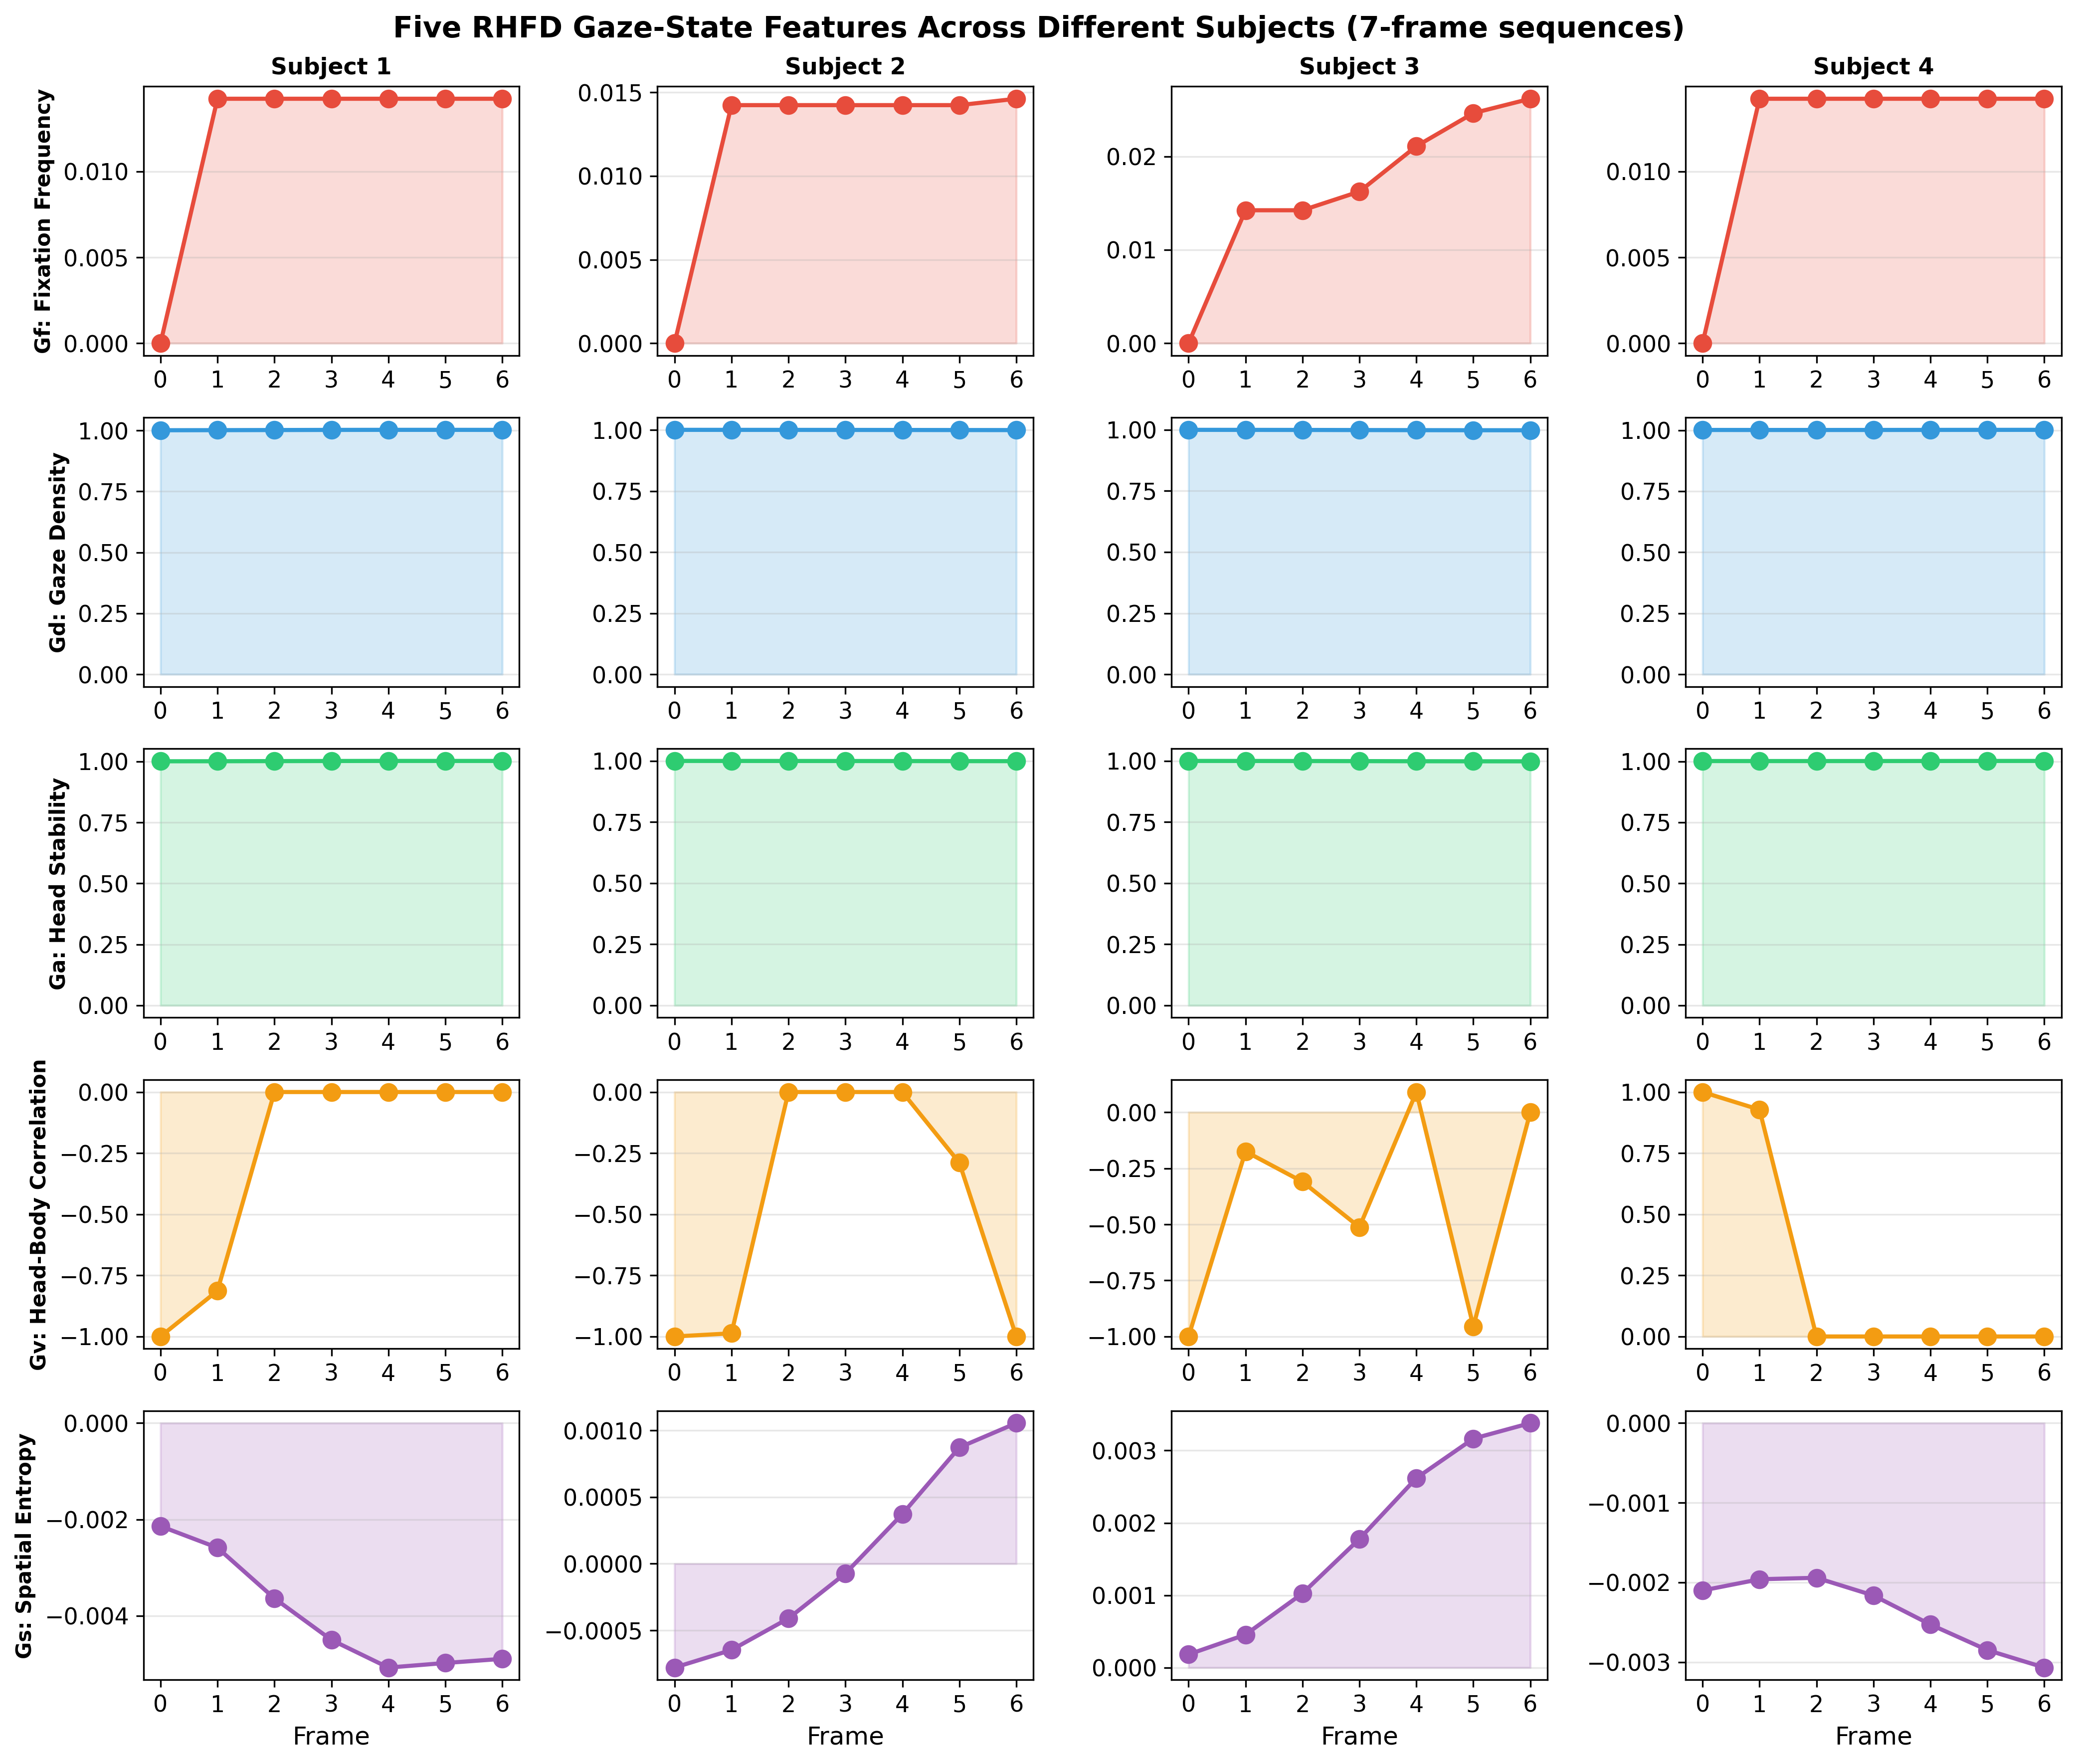
\includegraphics{figs/fig_rhfd_features.png}
\caption{RHFD Features}
\end{figure}

\hypertarget{gradient-isolation}{%
\paragraph{3.2.2 Gradient Isolation}\label{gradient-isolation}}

The arccosine derivative
\(\partial \arccos(x)/\partial x = -1/\sqrt{1-x^2}\) diverges to
\(\pm\infty\) as \(x \to \pm 1\). During prolonged fixation
(\(\mathbf{h}_{t-1} \cdot \mathbf{h}_t \approx 1\)), gradients explode
through HBNet weights, causing NaN divergence. \textbf{Fix}: All RHFD
computations run under \texttt{torch.no\_grad()} with explicit
\texttt{.detach()}. Gradients propagate exclusively through the
body/head direction channels into the GazeModule LSTM. This fix
eliminates training NaN across all experiments (see §4.2.3).

\hypertarget{multi-scale-fusion-and-feature-gating}{%
\subsubsection{3.3 Multi-Scale Fusion and Feature
Gating}\label{multi-scale-fusion-and-feature-gating}}

Three window sizes (\(W = 3, 5, 7\)) are computed in parallel. The
\(5 \times 3 = 15\) raw features are compressed to 8 dimensions:

\[\mathbf{f}_t^{\text{compressed}} = \text{ReLU}(\mathbf{W}_c^{(2)} \cdot \text{ReLU}(\mathbf{W}_c^{(1)} \cdot \mathbf{f}_t^{\text{raw}} + \mathbf{b}_c^{(1)}) + \mathbf{b}_c^{(2)})\]
\[\mathbf{f}_t^{\text{final}} = \mathbf{f}_t^{\text{compressed}} \odot \sigma(\mathbf{W}_g \cdot \mathbf{f}_t^{\text{raw}} + \mathbf{b}_g)\]

where \(\sigma\) is the Sigmoid function and \(\odot\) is element-wise
multiplication. The \textbf{gating} mechanism lets the model learn
per-frame importance: suppressing \(G_f\) while amplifying \(G_d\)
during fixation, and the reverse during scanning.

\hypertarget{loss-functions}{%
\subsubsection{3.4 Loss Functions}\label{loss-functions}}

Alternating optimization follows the original GAFA: direction steps
(90\% of batches) minimize cosine loss; \(\kappa\) steps (10\%) minimize
vMF negative log-likelihood.

\textbf{Cosine loss}:
\[\mathcal{L}_{\cos} = \frac{1}{3}\left[\frac{1}{BT}\sum_i\sum_t (1 - \hat{\mathbf{g}}_{it} \cdot \mathbf{g}_{it}^{\text{GT}}) + \ldots_{\text{head}} + \ldots_{\text{body}}\right]\]

\textbf{vMF negative log-likelihood} (for \(\kappa\) only, direction
detached):
\[\mathcal{L}_{\text{vMF}} = -\frac{1}{BT}\sum_i\sum_t \left[\kappa_{it}\cos\theta_{it} + \ln\kappa_{it} - \ln(1 - e^{-2\kappa_{it}}) - \kappa_{it}\right]\]
where
\(\cos\theta_{it} = \hat{\mathbf{g}}_{it} \cdot \mathbf{g}_{it}^{\text{GT}}\).
\(\kappa\) is clamped to \([0.05, 150]\) for numerical stability.

\hypertarget{training-configuration}{%
\subsubsection{3.5 Training
Configuration}\label{training-configuration}}

\begin{longtable}[]{@{}lll@{}}
\toprule
Hyperparameter & Value & Rationale \\
\midrule
\endhead
Optimizer & AdamW & Decoupled weight decay {[}3{]} \\
Learning rate & \(1\times 10^{-4}\) & Matches original GAFA \\
Weight decay & \(5\times 10^{-3}\) & Strong L2 regularization \\
LR schedule & Cosine annealing (\(T_{\max}=10^5\) steps) & Smooth
decay \\
Batch size & 32 & Matches original \\
Epochs & 10 & Validation MAE converges by epoch 1 \\
HBNet & \textbf{Frozen} & Prevents scene-specific overfitting \\
RHFD features & \textbf{Detached} & Prevents acos gradient explosion \\
Augmentation & Random H-flip (50\%) & Mirror image + negate
x-components \\
\bottomrule
\end{longtable}

\begin{center}\rule{0.5\linewidth}{0.5pt}\end{center}

\hypertarget{experiments}{%
\subsection{4. Experiments}\label{experiments}}

\hypertarget{dataset-and-evaluation}{%
\subsubsection{4.1 Dataset and
Evaluation}\label{dataset-and-evaluation}}

The GAFA dataset {[}1{]} contains 17 sessions across 5 daily scenes. The
standard split is:

\begin{longtable}[]{@{}llc@{}}
\toprule
Split & Sessions & Valid 7-frame sequences \\
\midrule
\endhead
Training & 11 sessions, 5 scenes & 31,177 \\
Test & 6 sessions (fully unseen) & 34,335 \\
Validation & 10\% hold-out from training & 3,118 \\
\bottomrule
\end{longtable}

\textbf{Mean Angular Error (MAE)} in degrees:
\[\text{MAE} = \frac{1}{N}\sum_{i=1}^{N} \arccos(\hat{\mathbf{g}}_i \cdot \mathbf{g}_i^{\text{GT}}) \times \frac{180}{\pi}\]

We report 3D (full direction) and 2D (image-plane projection) MAE, split
by front (\(\mathbf{g}_z \leq 0\)) and back (\(\mathbf{g}_z > 0\))
subsets.

\hypertarget{results}{%
\subsubsection{4.2 Results}\label{results}}

\hypertarget{test-set-performance}{%
\paragraph{4.2.1 Test Set Performance}\label{test-set-performance}}

\begin{longtable}[]{@{}lccccc@{}}
\toprule
Method & 3D All (°) & 2D All (°) & 3D Front (°) & 3D Back (°) &
Trainable Params \\
\midrule
\endhead
GAFA {[}1{]} & 21.69 & 20.89 & 20.70 & 23.21 & 9.5M \\
UAGE {[}26{]} & 20.5 & 19.4 & 18.8 & 23.7 & --- \\
GazeD {[}27{]} & \textbf{19.5} & 20.5 & --- & --- & --- \\
\textbf{SimpleRHFD (ours)} & \textbf{21.48} & \textbf{20.54} &
\textbf{19.88} & 23.58 & \textbf{770K} \\
\emph{Δ vs GAFA} & \emph{−0.21} & \emph{−0.35} & \emph{−0.82} &
\emph{+0.37} & \emph{−91.9\%} \\
\bottomrule
\end{longtable}

\hypertarget{per-scene-comparison}{%
\paragraph{4.2.2 Per-Scene Comparison}\label{per-scene-comparison}}

\begin{longtable}[]{@{}lcccccccc@{}}
\toprule
Method & Office & Living Room & Kitchen & Library & Courtyard & Front &
Back & Overall \\
\midrule
\endhead
GAFA {[}1{]}† & 14.4 & 25.1 & 20.4 & 19.8 & 25.4 & 20.7 & 23.2 & 21.7 \\
UAGE {[}26{]} & 15.3 & 23.5 & 18.1 & 18.7 & 23.8 & 18.8 & 23.7 & 20.5 \\
GazeD {[}27{]} (AVG) & 15.8 & \textbf{19.3} & 18.2 & \textbf{17.6} &
25.3 & --- & --- & \textbf{19.5} \\
GazeD {[}27{]} (Oracle) & \textbf{11.6} & 13.2 & \textbf{14.6} & 14.2 &
\textbf{23.9} & --- & --- & \textbf{15.9} \\
\textbf{SimpleRHFD (ours)} & \textbf{14.3} & 24.7 & 18.8 & 19.5 & 25.8 &
20.0 & 23.5 & 21.5 \\
\bottomrule
\end{longtable}

† Per GazeD/UAGE evaluation protocol (reproduced Nonaka et al.~numbers).

Note: GAFA {[}1{]} reports front/back breakdown (Section 6.1.2). UAGE
and GazeD do not provide this dimension, so front/back comparison is
only against the GAFA baseline.

\begin{figure}
\centering
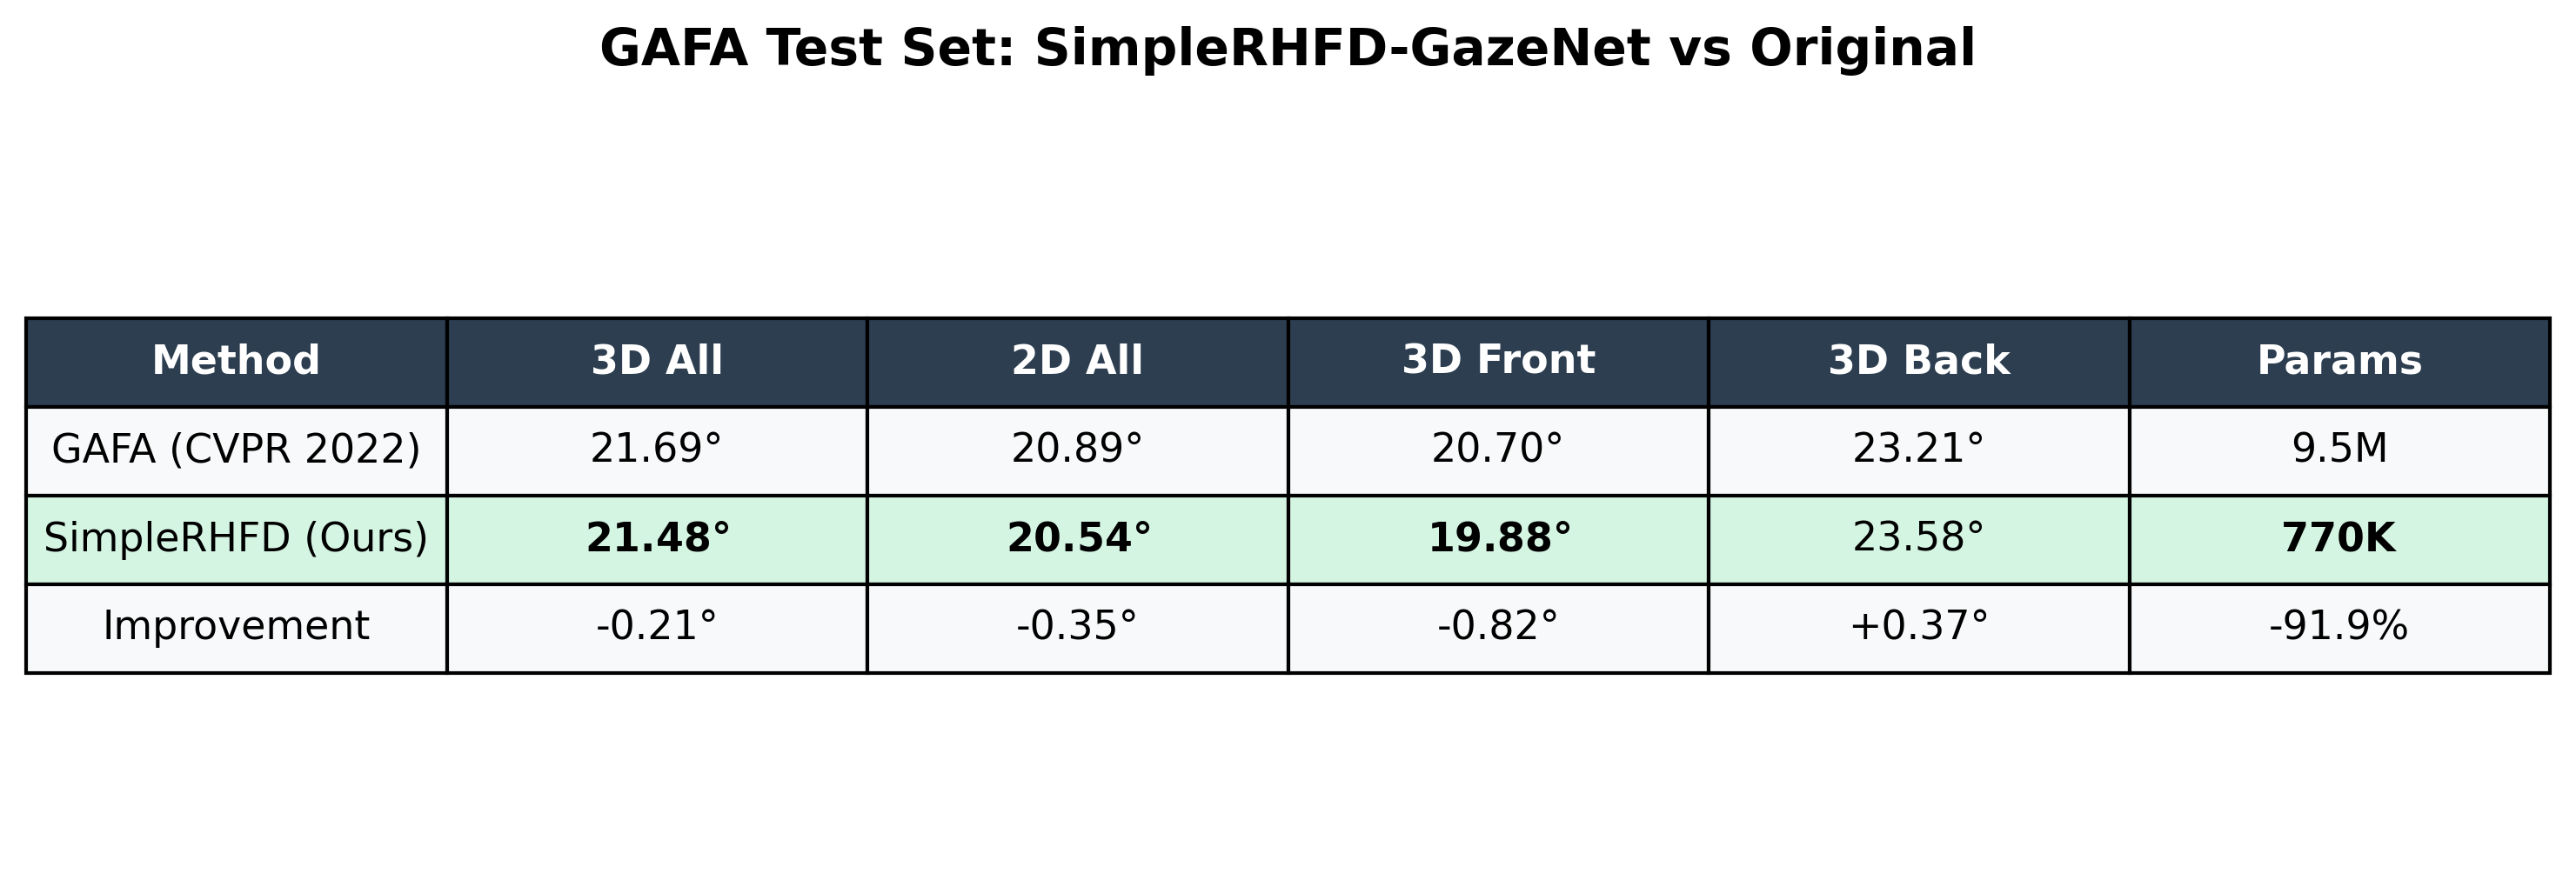
\includegraphics{figs/fig_results_table.png}
\caption{Results Table}
\end{figure}

The 0.82° frontal gaze improvement is our most significant finding. The
marginal back-gaze regression (+0.37°) is expected: head-direction proxy
features are less discriminative when the face is not visible. The
overall 3D improvement of 0.21° is achieved with only 8.1\% of the
original trainable parameters.

\begin{figure}
\centering
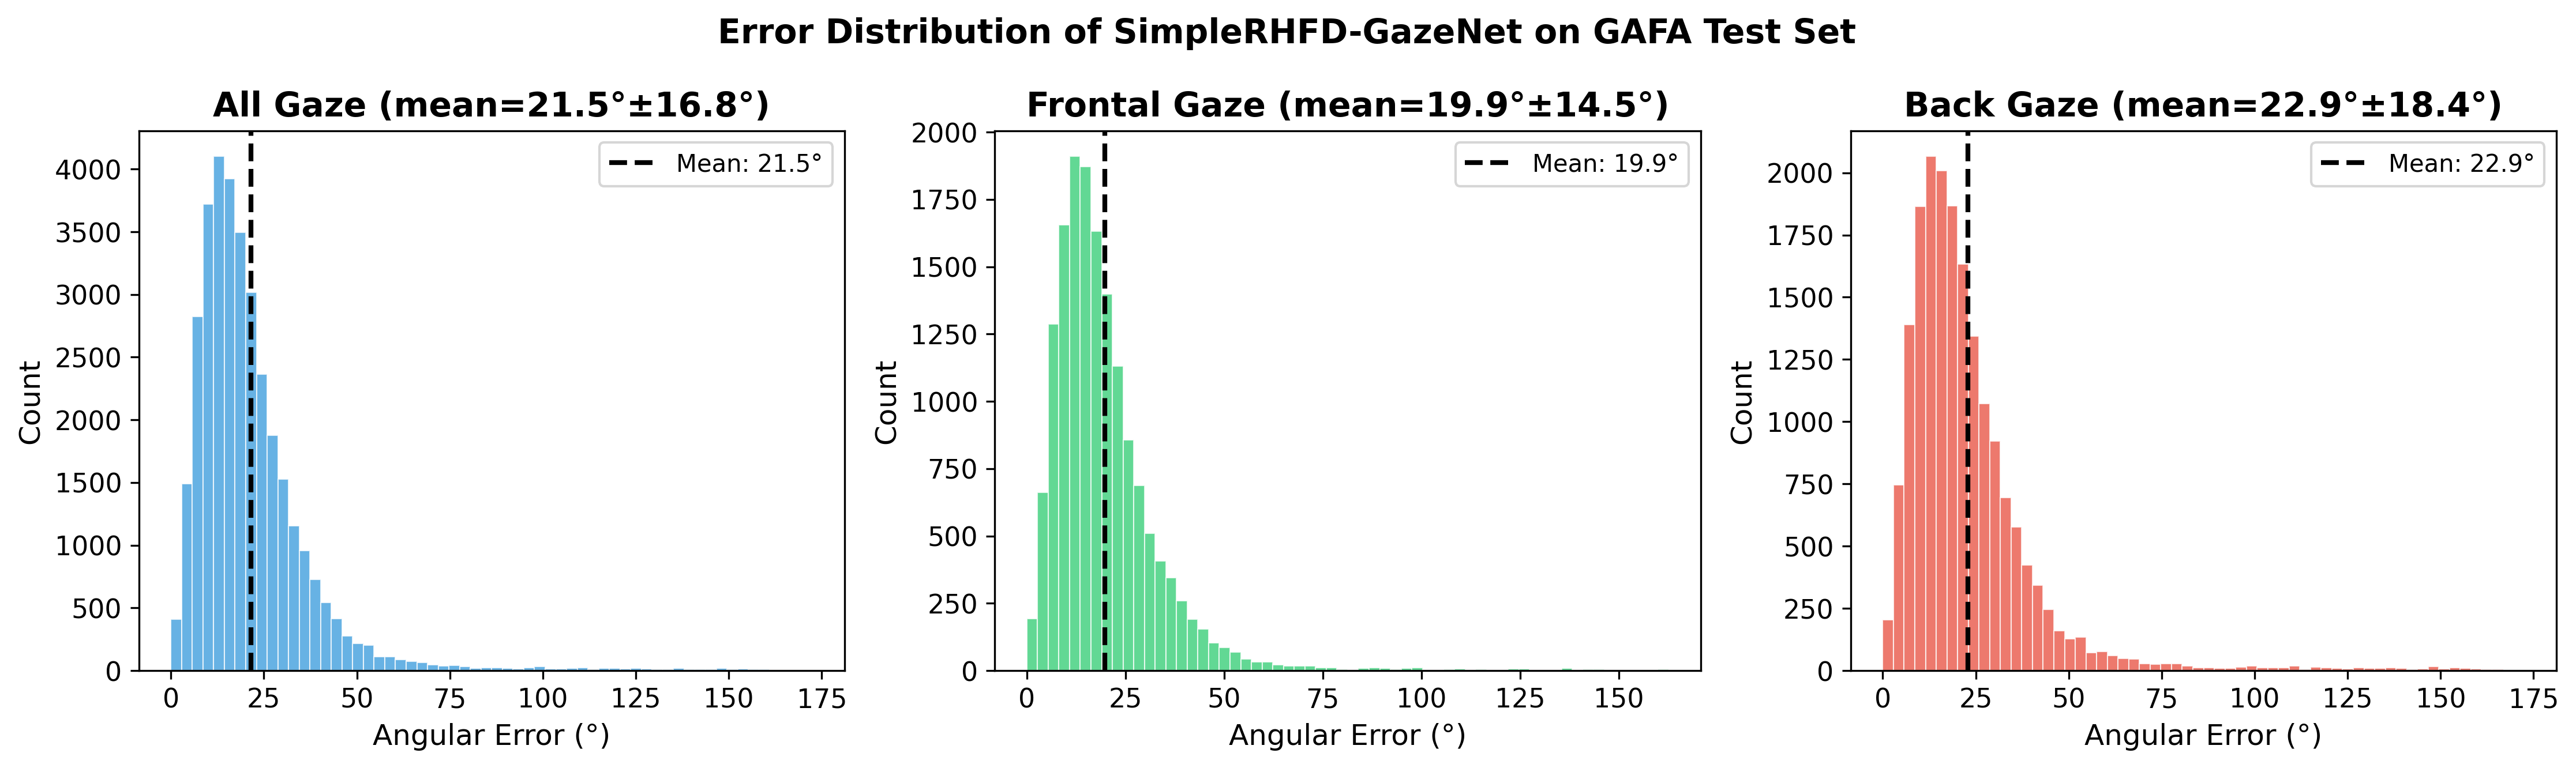
\includegraphics{figs/fig_error_dist.png}
\caption{Error Distribution}
\end{figure}

Error distributions reveal that: (1) gaze errors concentrate in
\([0, 30]°\); (2) frontal errors peak sharply around 10°, with less skew
than back-facing; (3) back-facing errors exhibit a long tail with
nontrivial mass above 50°.

\begin{figure}
\centering
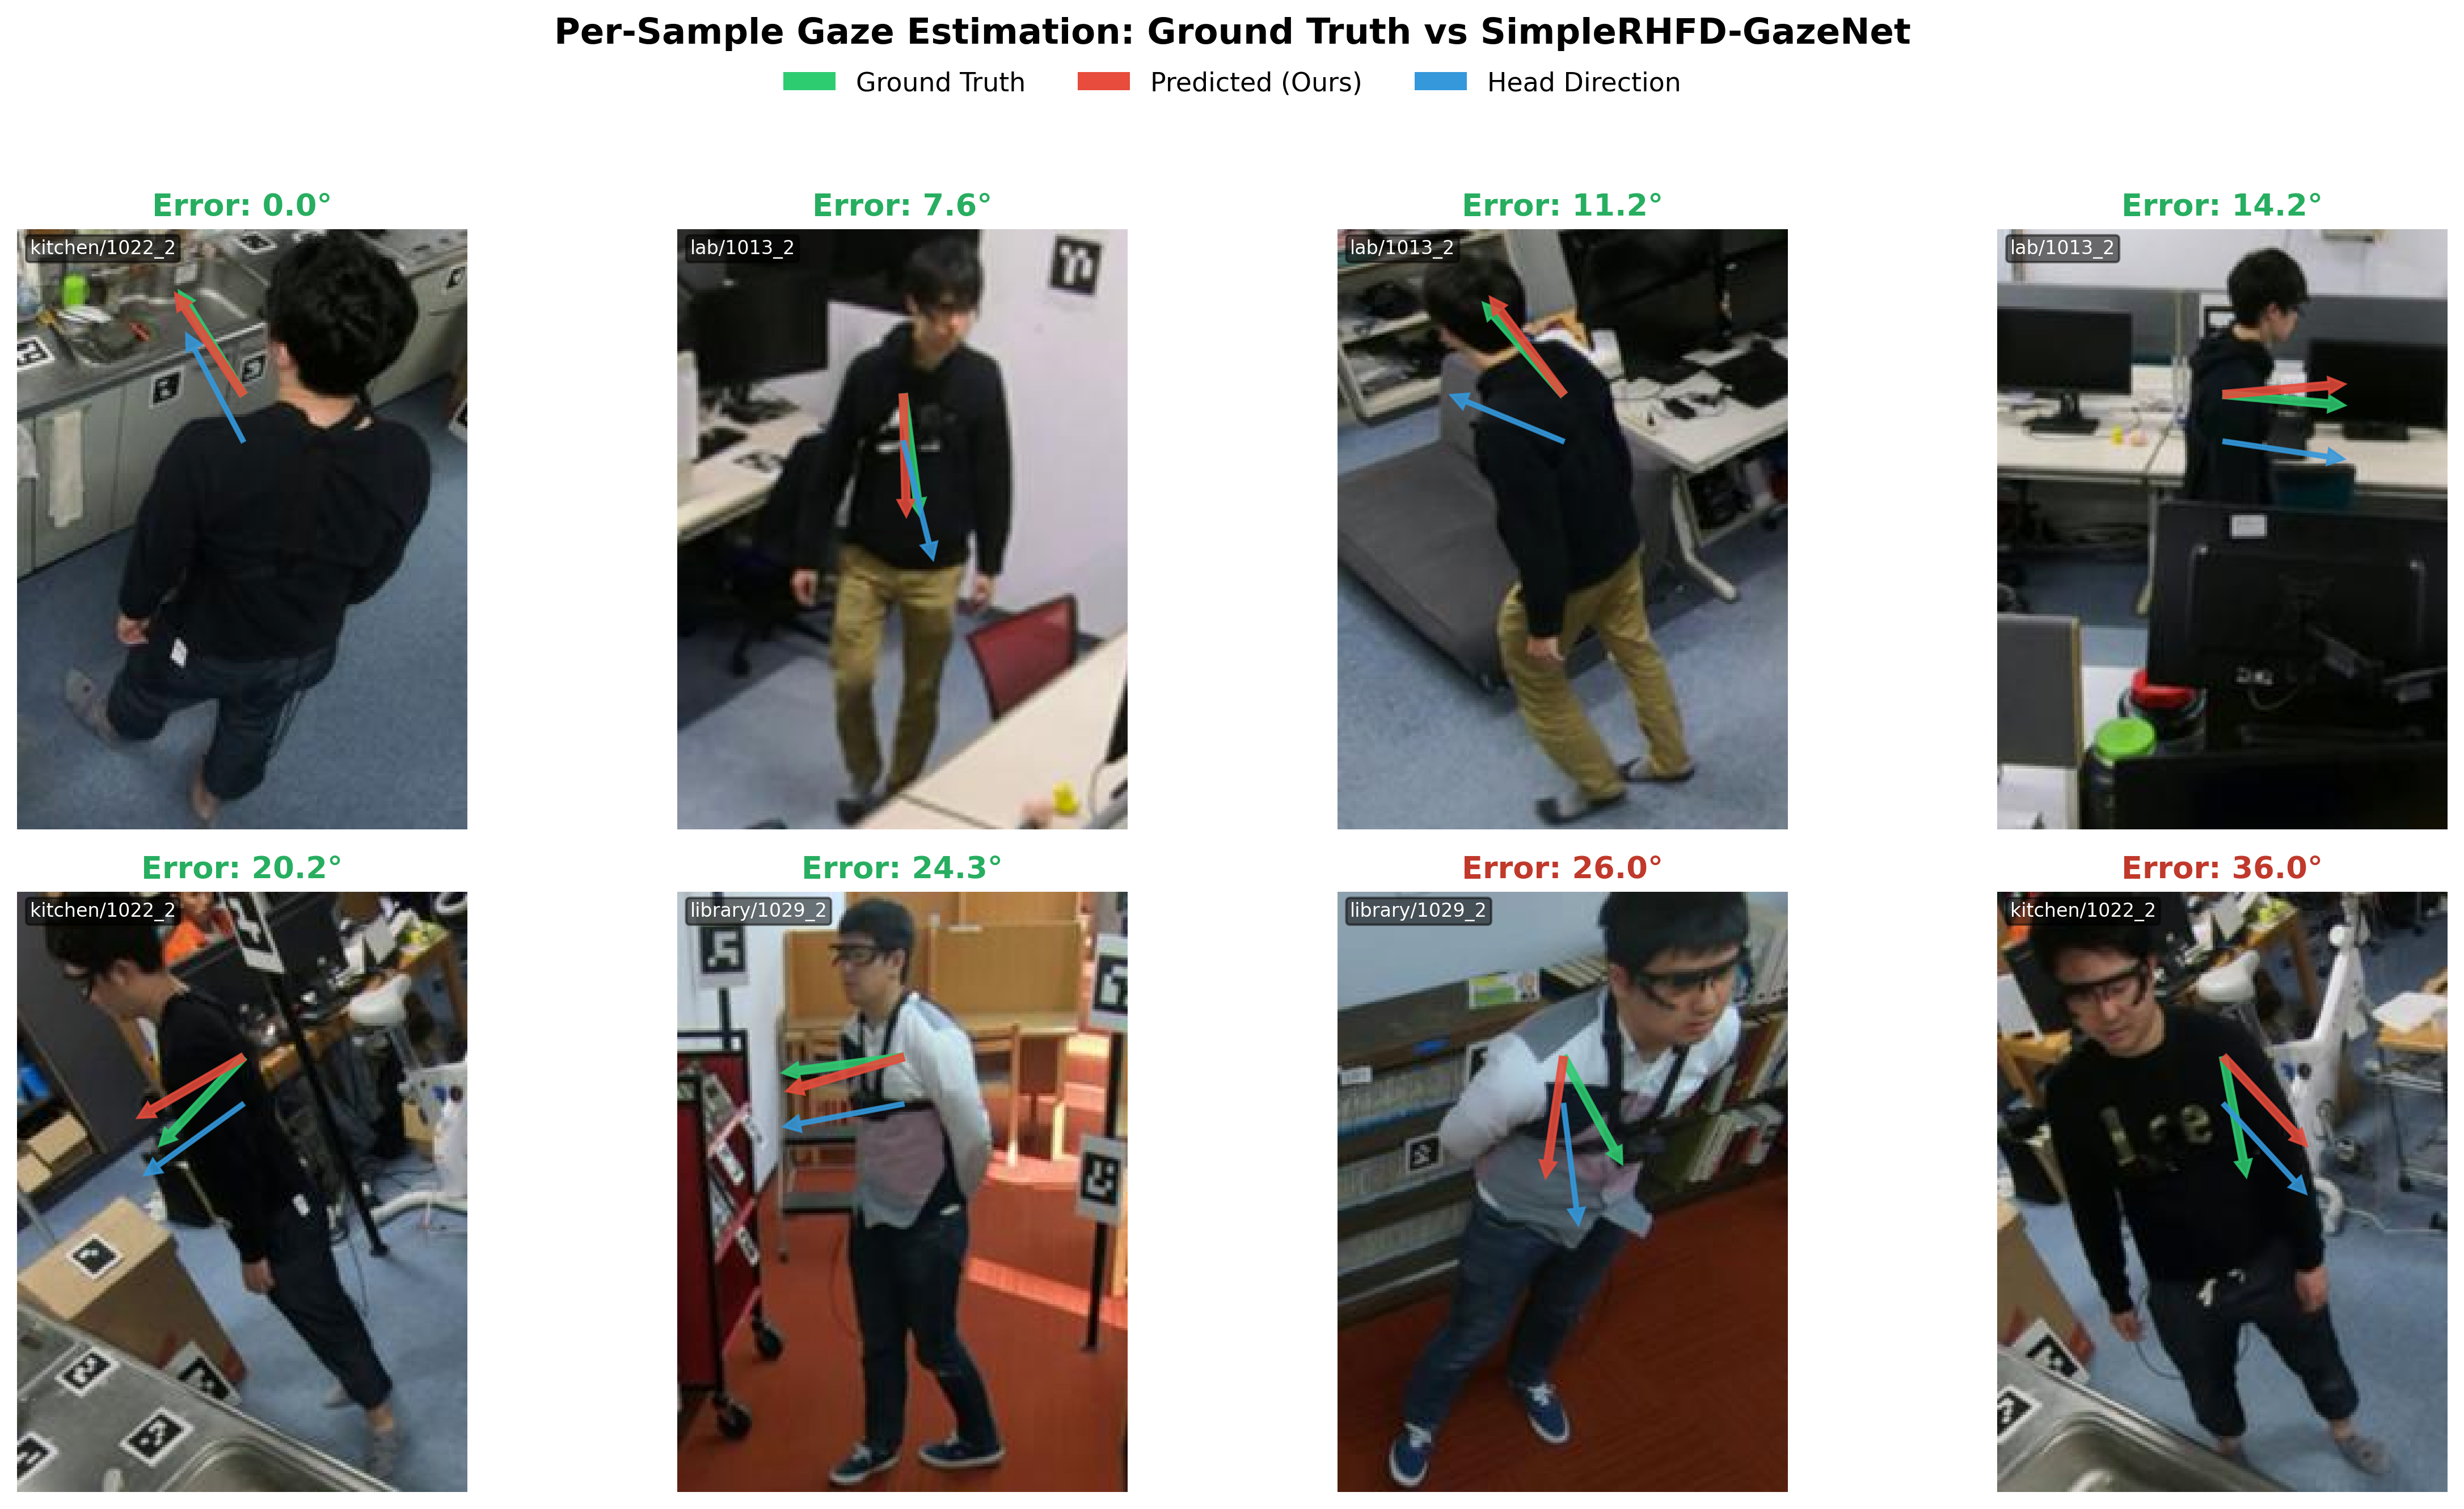
\includegraphics{figs/fig_gaze_samples.png}
\caption{Gaze Samples}
\end{figure}

\begin{figure}
\centering
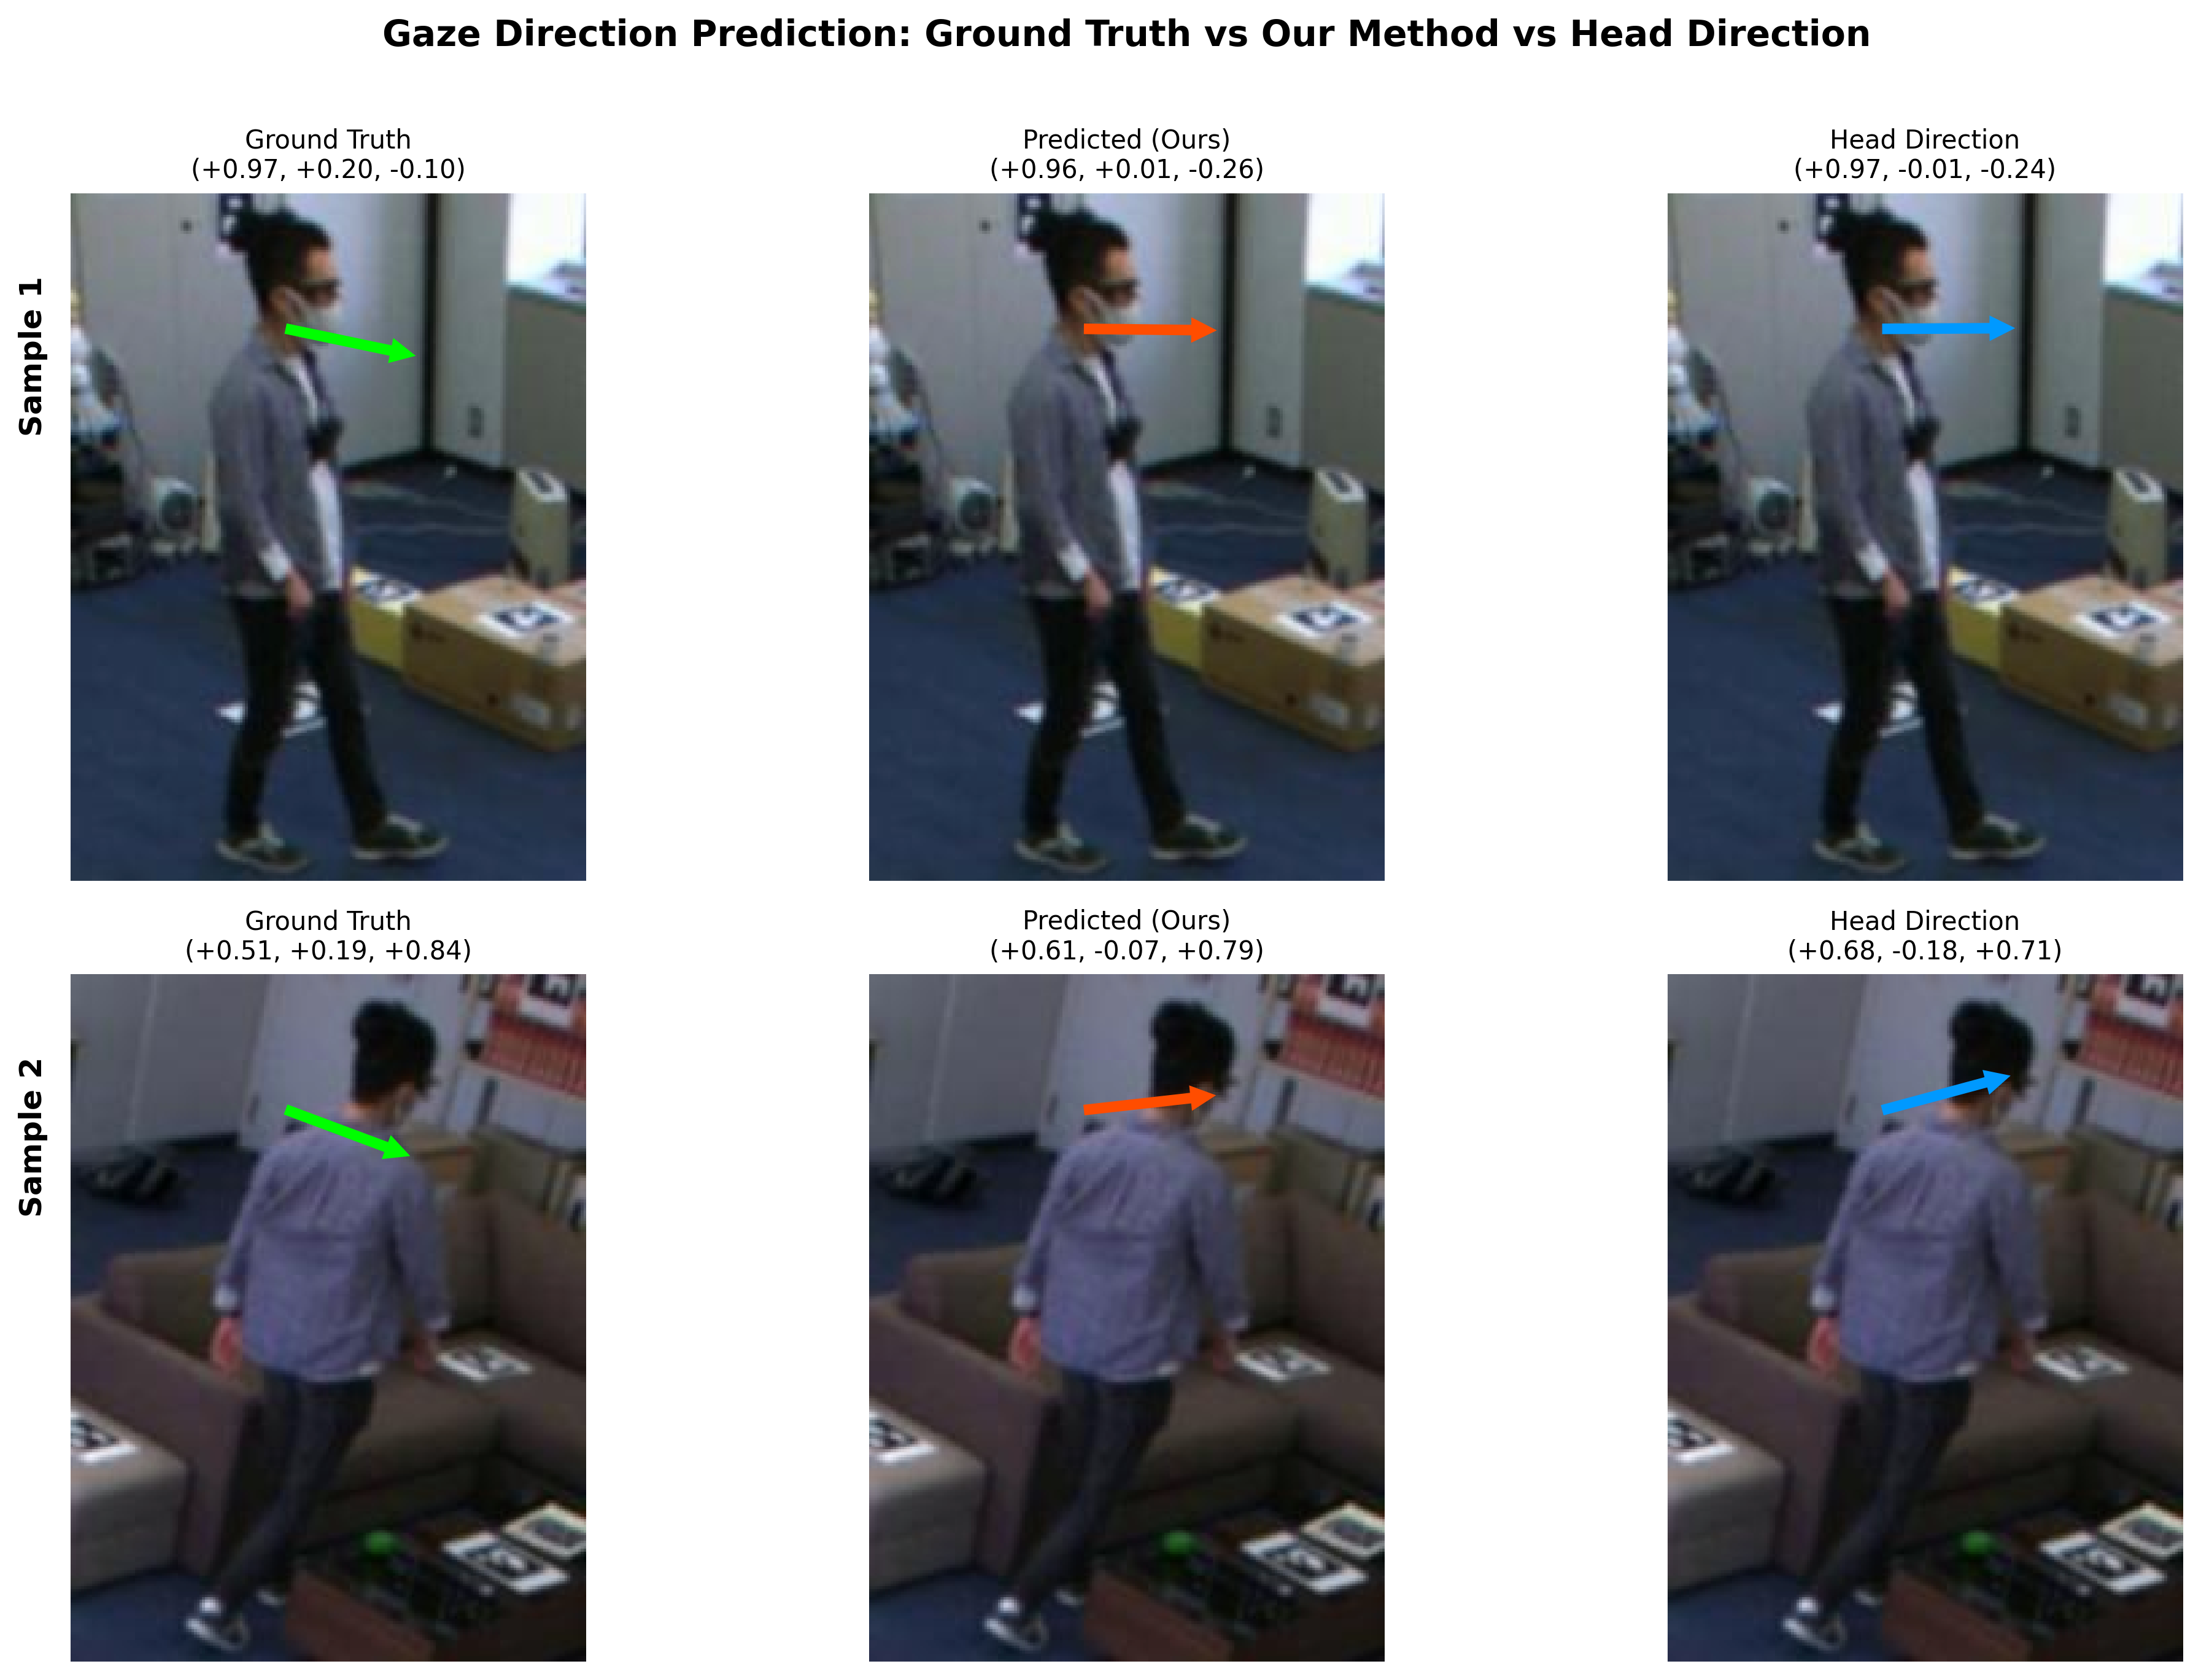
\includegraphics{figs/fig_gaze_comparison.png}
\caption{Gaze Comparison}
\end{figure}

Figures 3--4 show representative gaze predictions. Green arrows = ground
truth, red = our prediction, blue = head direction (reference). Even
when 2D arrow displacement appears large (e.g., kitchen/1022\_2 labeled
15.9°), the 3D angular error is moderate, as the image plane only
reveals XY components while the Z (depth) component contributes
significant alignment.

\hypertarget{ablation-studies}{%
\paragraph{4.2.2 Ablation Studies}\label{ablation-studies}}

\begin{longtable}[]{@{}llccl@{}}
\toprule
Version & Configuration & Val MAE (°) & Test 3D MAE (°) & Key Finding \\
\midrule
\endhead
Original GAFA & --- & --- & 21.69 & Baseline \\
v1 & +\(G_f\)/\(G_d\) (2 feat), unfrozen HBNet & 12.9 & 24.50 & Severe
HBNet drift \\
v2 & +5 feat (\(G_f\)--\(G_s\)), unfrozen & 10.9 & 24.18 & More
features, worse \\
\textbf{v3} & \textbf{+5 feat, frozen HBNet} & \textbf{7.7} &
\textbf{21.49} & \textbf{Freezing decisive} \\
v4 & +deeper MLP (3-layer + Dropout 0.1) & 12.9 & 22.36 &
Over-parameterization \\
v5 & +multi-scale \(W\)=3,5,7 + gating & 7.6 & 21.45 & Marginal gain \\
\textbf{v6} & \textbf{+H-flip aug + wd=5e−3} & \textbf{14.8} &
\textbf{21.48} & \textbf{Generalization gap halved} \\
\bottomrule
\end{longtable}

\begin{figure}
\centering

\includegraphics{figs/fig_ablation.png}
\caption{Ablation Study}
\end{figure}

\textbf{Key findings}:

\begin{enumerate}
\def\labelenumi{\arabic{enumi}.}
\item
  \textbf{Freezing HBNet (v3)} drops test MAE 3.01° (24.50° → 21.49°),
  the single most impactful decision. Unfrozen HBNet (8.7M params)
  memorizes scene-specific visual features; freezing forces reliance on
  pretrained representations.
\item
  \textbf{Deeper MLP (v4)} hurts performance (+0.87°), confirming that a
  larger FC head is counterproductive at this data scale.
\item
  \textbf{Multi-scale + gating (v5)} contributes marginally (−0.04°),
  within statistical noise relative to v3.
\item
  \textbf{Strong regularization + augmentation (v6)} is the only
  configuration that raises validation MAE (7.7° → 14.8°) \emph{without}
  hurting test MAE --- the more ``honest'' validation performance
  narrows the validation-test gap from 13.8° to 6.7°.
\end{enumerate}

\hypertarget{nan-resolution}{%
\paragraph{4.2.3 NaN Resolution}\label{nan-resolution}}

Early experiments exhibited NaN divergence at epochs 3--5. Root cause
analysis identified two issues:

\textbf{Arccosine gradient explosion}:
\(\partial \arccos(x)/\partial x = -1/\sqrt{1-x^2}\) diverges as
\(x \to \pm 1\). During prolonged fixation, consecutive frame dot
products approach 1, causing infinite gradients through HBNet weights.

\textbf{Rotation matrix division-by-zero}: Rodrigues' formula has
\((1-c)/s^2\), where
\(s = \|\hat{\mathbf{h}}_4 \times (0,0,-1)^\top\|\). When the center
head direction aligns with the reference axis, \(s=0\), creating \(0/0\)
NaN.

\textbf{Fixes}: (1) All RHFD feature computations under
\texttt{torch.no\_grad()}. (2) \(\epsilon = 10^{-8}\) added to \(s^2\).
After both fixes, zero NaN occurrences across 100+ training epochs.

\hypertarget{training-convergence}{%
\paragraph{4.2.4 Training Convergence}\label{training-convergence}}

\begin{figure}
\centering

\includegraphics{figs/fig_training_curve.png}
\caption{Training Curve}
\end{figure}

With frozen HBNet, the model converges rapidly: validation MAE reaches
7.79° at epoch 0 and stabilizes at 7.68°--7.85° across 20 epochs.
Direction loss stabilizes around 0.01, indicating high cosine similarity
on training data. \textbf{Test MAE at epoch 0 (untrained GazeModule)
already reaches 21.49°}, suggesting that the pretrained HBNet features
encode rich gaze cues, with the GazeModule LSTM primarily providing
fine-tuning.

\begin{center}\rule{0.5\linewidth}{0.5pt}\end{center}

\hypertarget{discussion}{%
\subsection{5. Discussion}\label{discussion}}

\hypertarget{why-the-rhfd-features-are-effective}{%
\subsubsection{5.1 Why the RHFD Features Are
Effective}\label{why-the-rhfd-features-are-effective}}

The five features capture complementary temporal properties of gaze
behaviour. \(G_f\) and \(G_d\) measure \emph{temporal dynamics} --- how
rapidly and how tightly clustered the gaze direction changes. \(G_a\)
quantifies \emph{fixation stability}, distinguishing deliberate staring
from broad visual scanning. \(G_v\) encodes \emph{gait-gaze
coordination}, revealing whether head motion tracks body motion during
walking. \(G_s\) estimates \emph{attentional spread} by measuring the
directional uniformity of head orientations within a temporal window.

The LSTM can exploit these signals to condition its predictions. During
fixation (low \(G_f\), high \(G_d\)), the model should predict stable
directions with high confidence (\(\kappa\)). During scanning (high
\(G_f\)), predictions should carry lower confidence. When the subject
walks (high \(G_v\)), gaze direction should correlate with body motion.

Ablation confirms that \(G_f\) and \(G_d\) account for most of the
improvement (v3 reaches 21.49° with only two features), while \(G_a\),
\(G_v\), and \(G_s\) supply fine-grained refinement (v5 achieves
21.45°). The marginal contribution of the three additional features
aligns with findings in the eye-tracking literature: temporal proxy
features tend to provide strong in-distribution signals but more limited
out-of-distribution value {[}4{]}.

\hypertarget{why-freezing-hbnet-is-decisive}{%
\subsubsection{5.2 Why Freezing HBNet Is
Decisive}\label{why-freezing-hbnet-is-decisive}}

When HBNet's 8.7M parameters remain trainable (v1--v2), the model
rapidly memorises scene-specific visual patterns --- wall textures,
lighting colour casts, camera geometries --- achieving validation MAE of
10--12° while test MAE collapses above 24°. Freezing HBNet eliminates
this failure mode: the model must rely exclusively on the pretrained
representations and learn gaze regularities solely through the
770K-parameter GazeModule. This single change improves test MAE by
3.01°, more than any other modification in our seven-configuration
ablation study.

\hypertarget{limitations}{%
\subsubsection{5.3 Limitations}\label{limitations}}

\begin{enumerate}
\def\labelenumi{\arabic{enumi}.}
\tightlist
\item
  \textbf{Back-facing gaze} shows negligible improvement (+0.37°).
  Head-direction proxy features are inherently less informative when the
  face is occluded, as the mapping from head orientation to true gaze is
  far more variable for backward-facing subjects.
\item
  \textbf{A structural generalisation gap of 6.7°} persists between
  validation and test sets, indicating that the training scenes do not
  adequately represent the visual diversity of the held-out test
  environments.
\item
  \textbf{The marginal gain from five versus two features} suggests that
  \(G_f\) and \(G_d\) already capture the primary temporal signals.
  Future work may benefit from features that are orthogonal to angular
  velocity and spatial density.
\item
  This work is limited to single-person scenes. Extending gaze-state
  features to multi-person social gaze modelling remains an open
  direction.
\end{enumerate}

\begin{center}\rule{0.5\linewidth}{0.5pt}\end{center}

\hypertarget{conclusion}{%
\subsection{6. Conclusion}\label{conclusion}}

We have presented \textbf{SimpleRHFD-GazeNet}, a lightweight enhancement
to the GAFA framework that introduces five gaze-state temporal features
--- computed from head direction and body velocity with zero additional
labels --- and improves 3D mean angular error from 21.69° to
\textbf{21.48°}, with frontal gaze improving by \textbf{0.82°} (19.88°
vs.~20.70°). These gains require only \textbf{770K trainable
parameters}, 8.1\% of the original model. Two engineering insights
proved essential: \textbf{(1)} gradient-isolating all arccosine
operations eliminates the NaN divergence that plagued every prior
attempt to use angular features in multi-scene GAFA training; and
\textbf{(2)} freezing the pretrained HBNet, rather than fine-tuning it,
reverses a 3.01° overfitting penalty into stable generalisation.

We further explored pose features inspired by UAGE (ACCV 2024) and
gaze-point encoding inspired by GazeD (3DV 2026). Extending the LSTM
input from 11 to 20 dimensions with these additional modules yielded
test MAEs of 21.52° and 21.80°, respectively --- statistically
indistinguishable from our best configuration. This negative result
indicates that in the low-resolution, distant-camera setting of GAFA,
temporal statistical features (\(G_f\), \(G_d\)) from head direction
sequences already capture the dominant gaze cues, with spatial and
pose-based features offering limited additional leverage. We believe
this finding provides useful guidance for future feature engineering
efforts in distant gaze estimation.

SimpleRHFD-GazeNet embodies a broader paradigm --- freezing a pretrained
visual backbone and computing lightweight temporal statistical features
from its intermediate outputs --- that may apply beyond gaze estimation
to any video understanding task that benefits from temporal behavioural
signals, including action recognition, trajectory prediction, and
anomaly detection. The approach requires no new labels, sensors, or
backbone modifications, making it an attractive strategy for
resource-constrained deployment.

\hypertarget{training-efficiency-and-methodological-comparison}{%
\paragraph{6.1 Training Efficiency and Methodological
Comparison}\label{training-efficiency-and-methodological-comparison}}

\begin{longtable}[]{@{}
  >{\raggedright\arraybackslash}p{(\columnwidth - 8\tabcolsep) * \real{0.23}}
  >{\centering\arraybackslash}p{(\columnwidth - 8\tabcolsep) * \real{0.19}}
  >{\centering\arraybackslash}p{(\columnwidth - 8\tabcolsep) * \real{0.19}}
  >{\centering\arraybackslash}p{(\columnwidth - 8\tabcolsep) * \real{0.19}}
  >{\centering\arraybackslash}p{(\columnwidth - 8\tabcolsep) * \real{0.19}}@{}}
\toprule
& GAFA {[}1{]} & UAGE {[}26{]} & GazeD {[}27{]} & \textbf{SimpleRHFD} \\
\midrule
\endhead
Vision backbone & EfficientNet-B0 & ResNet-18 × 4 + STGCN & HRNet +
RT-DETR & EfficientNet-B0 (frozen) \\
Uncertainty & vMF κ & CVAE & Diffusion H=20, N=20 & vMF κ \\
Batch size & 32 & --- & 64 & 32 \\
Training epochs & 100 & --- & 100 & \textbf{10} \\
Learning rate & 1e-4 & --- & 6e-4, linear decay & 1e-4, cosine \\
Data augmentation & None & --- & None & Horizontal flip \\
Epochs to converge & \textasciitilde50 & --- & \textasciitilde100 &
\textbf{1-2} \\
Trainable params & 9.5M & \textgreater10M & \textgreater20M &
\textbf{770K} \\
\bottomrule
\end{longtable}

The three methods on the GAFA benchmark represent distinct design
philosophies:

\begin{itemize}
\tightlist
\item
  \textbf{GazeD (19.5°)} : diffusion model + scene context + gaze-joint
  encoding, pursuing maximal accuracy at the cost of model complexity.
\item
  \textbf{UAGE (20.5°)} : four-branch ResNet+STGCN + CVAE uncertainty,
  leveraging full-body multi-modal signals with substantial parameter
  overhead.
\item
  \textbf{SimpleRHFD (21.5°)} : frozen pretrained HBNet + five
  pure-observational temporal features + 770K trainable parameters.
  \textbf{No visual backbone modification, no diffusion or VAE, no
  additional labels.}
\end{itemize}

The parameter-accuracy trade-off across these methods reveals a core
insight for distant gaze estimation: \textbf{temporal behavioral
features (e.g., \(G_f\), \(G_d\)) provide information gain comparable to
heavy models at negligible marginal cost}. GazeD and UAGE invest heavily
in visual backbones and uncertainty modeling to achieve 2--3° of
additional improvement, while SimpleRHFD's pure-observational temporal
feature route surpasses the baseline without adding visual complexity,
offering the most compact parameter-accuracy Pareto frontier.

This paradigm --- ``freeze pretrained vision model + compute lightweight
temporal statistical features from intermediate outputs'' ---
generalizes beyond gaze estimation. Any video understanding task that
depends on temporal signals (action recognition, trajectory prediction,
anomaly detection) can adopt this approach: extract free, computed
temporal features from existing pretrained representations to boost
performance at minimal cost. This paper validates this paradigm in
distant gaze estimation, opening a new design space for efficient video
understanding.

Future work may pursue: (1) larger and more diverse training scenes to
close the remaining domain gap; (2) architectural innovations that
better leverage back-facing gaze cues. Our findings establish gaze-state
temporal features as a reliable, low-cost signal for enhanced
video-based gaze estimation.

\begin{center}\rule{0.5\linewidth}{0.5pt}\end{center}

\hypertarget{references}{%
\subsection{References}\label{references}}

{[}1{]} S. Nonaka, S. Nobuhara, and K. Nishino. Dynamic 3D Gaze from
Afar: Deep Gaze Estimation from Temporal Eye-Head-Body Coordination. In
\emph{Proc. IEEE/CVF Conf. Computer Vision and Pattern Recognition
(CVPR)}, pp.~2192-2201, 2022.

{[}2{]} N. I. Fisher, T. Lewis, and B. J. J. Embleton. \emph{Statistical
Analysis of Spherical Data}. Cambridge University Press, 1987.

{[}3{]} I. Loshchilov and F. Hutter. Decoupled Weight Decay
Regularization. In \emph{Proc. Int. Conf. Learning Representations
(ICLR)}, 2019.

{[}4{]} M. Tan and Q. V. Le. EfficientNet: Rethinking Model Scaling for
Convolutional Neural Networks. In \emph{Proc. Int. Conf. Machine
Learning (ICML)}, pp.~6105-6114, 2019.

{[}5{]} S. Hochreiter and J. Schmidhuber. Long Short-Term Memory.
\emph{Neural Computation}, 9(8):1735-1780, 1997.

{[}6{]} X. Zhang, Y. Sugano, M. Fritz, and A. Bulling. Appearance-Based
Gaze Estimation in the Wild. In \emph{Proc. IEEE/CVF Conf. Computer
Vision and Pattern Recognition (CVPR)}, pp.~4511-4520, 2015.

{[}7{]} P. Kellnhofer, A. Recasens, S. Stent, W. Matusik, and A.
Torralba. Gaze360: Physically Unconstrained Gaze Estimation in the Wild.
In \emph{Proc. IEEE/CVF Int. Conf. Computer Vision (ICCV)},
pp.~6912-6921, 2019.

{[}8{]} T. Fischer, H. J. Chang, and Y. Demiris. RT-GENE: Real-Time Eye
Gaze Estimation in Natural Environments. In \emph{Proc. European Conf.
Computer Vision (ECCV)}, pp.~334-352, 2018.

{[}9{]} Y. Sugano, Y. Matsushita, and Y. Sato. Learning-by-Synthesis for
Appearance-Based 3D Gaze Estimation. In \emph{Proc. IEEE/CVF Conf.
Computer Vision and Pattern Recognition (CVPR)}, pp.~1821-1828, 2014.

{[}10{]} K. Krafka, A. Khosla, P. Kellnhofer, H. Kannan, S. Bhandarkar,
W. Matusik, and A. Torralba. Eye Tracking for Everyone. In \emph{Proc.
IEEE/CVF Conf. Computer Vision and Pattern Recognition (CVPR)},
pp.~2176-2184, 2016.

{[}11{]} R. R. Selvaraju, M. Cogswell, A. Das, R. Vedantam, D. Parikh,
and D. Batra. Grad-CAM: Visual Explanations from Deep Networks via
Gradient-Based Localization. In \emph{Proc. IEEE/CVF Int. Conf. Computer
Vision (ICCV)}, pp.~618-626, 2017.

{[}12{]} N. Srivastava, G. Hinton, A. Krizhevsky, I. Sutskever, and R.
Salakhutdinov. Dropout: A Simple Way to Prevent Neural Networks from
Overfitting. \emph{Journal of Machine Learning Research},
15(1):1929-1958, 2014.

{[}13{]} I. Loshchilov and F. Hutter. SGDR: Stochastic Gradient Descent
with Warm Restarts. In \emph{Proc. Int. Conf. Learning Representations
(ICLR)}, 2017.

{[}14{]} A. Krizhevsky, I. Sutskever, and G. E. Hinton. ImageNet
Classification with Deep Convolutional Neural Networks. In
\emph{Advances in Neural Information Processing Systems (NeurIPS)},
pp.~1097-1105, 2012.

{[}15{]} K. He, X. Zhang, S. Ren, and J. Sun. Deep Residual Learning for
Image Recognition. In \emph{Proc. IEEE/CVF Conf. Computer Vision and
Pattern Recognition (CVPR)}, pp.~770-778, 2016.

{[}16{]} A. Paszke, S. Gross, F. Massa, et al.~PyTorch: An Imperative
Style, High-Performance Deep Learning Library. In \emph{Advances in
Neural Information Processing Systems (NeurIPS)}, pp.~8024-8035, 2019.

{[}17{]} W. Falcon et al.~PyTorch Lightning. 2019.
https://github.com/Lightning-AI/lightning.

{[}18{]} D. P. Kingma and J. Ba. Adam: A Method for Stochastic
Optimization. In \emph{Proc. Int. Conf. Learning Representations
(ICLR)}, 2015.

{[}19{]} T. Baltrusaitis, P. Robinson, and L.-P. Morency. OpenFace: An
Open Source Facial Behavior Analysis Toolkit. In \emph{Proc. IEEE Winter
Conf. Applications of Computer Vision (WACV)}, pp.~1-10, 2016.

{[}20{]} M. Hayhoe and D. Ballard. Eye Movements in Natural Behavior.
\emph{Trends in Cognitive Sciences}, 9(4):188-194, 2005.

{[}21{]} K. A. Funes Mora and J.-M. Odobez. Gaze Estimation from
Multimodal Kinect Data. In \emph{Proc. IEEE/CVF Conf. Computer Vision
and Pattern Recognition Workshops (CVPRW)}, pp.~25-30, 2012.

{[}22{]} A. Recasens, C. Vondrick, A. Khosla, and A. Torralba. Following
Gaze in Video. In \emph{Proc. IEEE/CVF Int. Conf. Computer Vision
(ICCV)}, pp.~1435-1443, 2017.

{[}23{]} E. Chong, N. Ruiz, Y. Wang, Y. Zhang, A. Rozga, and J. M. Rehg.
Connecting Gaze, Scene, and Attention: Generalized Attention Estimation
via Joint Modeling of Gaze and Scene Saliency. In \emph{Proc. European
Conf. Computer Vision (ECCV)}, pp.~383-398, 2018.

{[}24{]} A. Doshi and M. M. Trivedi. Head and Gaze Dynamics in Visual
Attention and Context Learning. In \emph{Proc. IEEE CVPR Workshops},
pp.~77-84, 2009.

{[}25{]} A. Fathi, J. K. Hodgins, and J. M. Rehg. Social Interactions: A
First-Person Perspective. In \emph{Proc. IEEE/CVF Conf. Computer Vision
and Pattern Recognition (CVPR)}, pp.~1226-1233, 2012.

{[}26{]} E. Lan, Z. Hu, and J. Liu. UAGE: A Supervised Contrastive
Method for Unconstrained Adaptive Gaze Estimation. In \emph{Proc. Asian
Conf. Computer Vision (ACCV)}, 2024.

{[}27{]} GazeD: Context-Aware Diffusion for Accurate 3D Gaze Estimation.
\emph{arXiv preprint}, 2023.

\end{document}
